\documentclass[preprint,12pt,3p]{elsarticle}

\usepackage{amsmath,amssymb,amsfonts}
\usepackage{booktabs}
\usepackage{siunitx}
\usepackage{graphicx}
\usepackage{hyperref}
\usepackage{cleveref}
\usepackage{tabularx}

\journal{Aerospace Science and Technology}

\newcommand{\code}[1]{\texttt{\detokenize{#1}}}
\newcommand{\Grms}{\text{G}_{\text{rms}}}
\newcommand{\Grmspay}{G_{\text{rms, pay}}}
\newcommand{\Grmsbase}{G_{\text{rms, base}}}
\newcommand{\rail}{8.5 \times 8.5\text{ mm}}

\begin{document}

\begin{frontmatter}

\title{Passive Vibration Isolation and Random Dynamic Launch Qualification of 3D-Printed Auxetic Spacecraft Chassis}

\author[uesc]{Gabriel Marques de Andrade\corref{cor1}}
\ead{gabriel.andrade@uesc.br}

\author[uesc]{Nila C. F. L. Medeiros}
\ead{nila.medeiros@uesc.br}

\cortext[cor1]{Corresponding author}
\address[uesc]{Department of Exact and Technological Sciences, State University of Santa Cruz (UESC), Rodovia Jorge Amado km 16, Ilh\'eus, BA 45662-900, Brazil}

\begin{abstract}
During rocket ascent and stage separation, containerized secondary payloads launched from standard tubular canisters, such as the Poly-Picosatellite Orbital Deployer (P-POD), are subjected to severe broadband vibroacoustic launch excitation governed by the NASA GSFC-STD-7000A General Environmental Verification Standard ($14.1\text{ G}_{\text{rms}}$ over $20\text{--}2000$~Hz). Conventional monolithic machined aluminum CubeSat chassis impose excessive structural mass fractions ($>25\text{--}35\%$) and exhibit virtually zero intrinsic mechanical damping, transmitting destructive acoustic energy directly into sensitive optical detectors and avionics stacks. In this investigation, we establish the elastodynamic modeling, passive vibration shielding performance, and formal spaceflight qualification of an additively manufactured 1U CubeSat chassis featuring 2D re-entrant auxetic metamaterials ($\nu_{\text{eff}} = -0.428$) fabricated via Laser Powder Bed Fusion (L-PBF) in aerospace-grade AlSi10Mg alloy. A high-order finite element elastodynamic pipeline orchestrated in Linux integrates Gmsh quadratic tetrahedral discretization (Tet10 with up to 342,800 nodes), dual open-source solvers (Code\_Aster Lanczos extraction and CalculiX verification), and full modal superposition random vibration synthesis (\code{DYNA_ALEA_MODAL}). Dual kinematic boundary conditions are modeled: shaker table clamped rails and canister-coupled flexible deployer rails ($k_s = 2.5 \times 10^6$~N/m). Under the full $14.1\text{ G}_{\text{rms}}$ NASA GEVS random vibration spectrum, the optimized auxetic chassis (\#28) acts as an intrinsic passive mechanical filter, achieving a remarkable $76.50\%$ ($-12.6$~dB) broadband acceleration attenuation at the payload mounting interface ($2.82\text{ G}_{\text{rms}}$ compared to $12.0\text{ G}_{\text{rms}}$ for the conventional solid baseline), while simultaneously reducing structural bus mass by $62.49\%$ ($0.116$~kg vs. $0.308$~kg). The fundamental natural frequency satisfies launch vehicle decoupling requirements ($f_1 = 579.6$~Hz clamped, $304.1$~Hz in-deployer, with $MS_{f_1} = +2.04$ over the NASA $100$~Hz threshold). Flight structural integrity is certified under stochastic $3\sigma$ peak stress ($\sigma_{3\sigma} = 166.91$~MPa, yielding $MS_{\text{yield}} = +0.102$ and $MS_{\text{ult}} = +0.455$) and benign Steinberg 3-band cumulative fatigue damage ($D = 0.0458 \ll 0.25$, ensuring a $5.4\times$ life factor). Linear elastic notch fracture mechanics confirms that the Mode I stress intensity range ($\Delta K_1^V = 1.12\text{ MPa}\sqrt{\text{m}}$) remains strictly below the threshold $\Delta K_{\text{th}} = 2.50\text{ MPa}\sqrt{\text{m}}$, proving that cellular auxetic architectures represent a flight-ready, multifunctional paradigm for small satellite structures.
\end{abstract}

\begin{graphicalabstract}
\centering
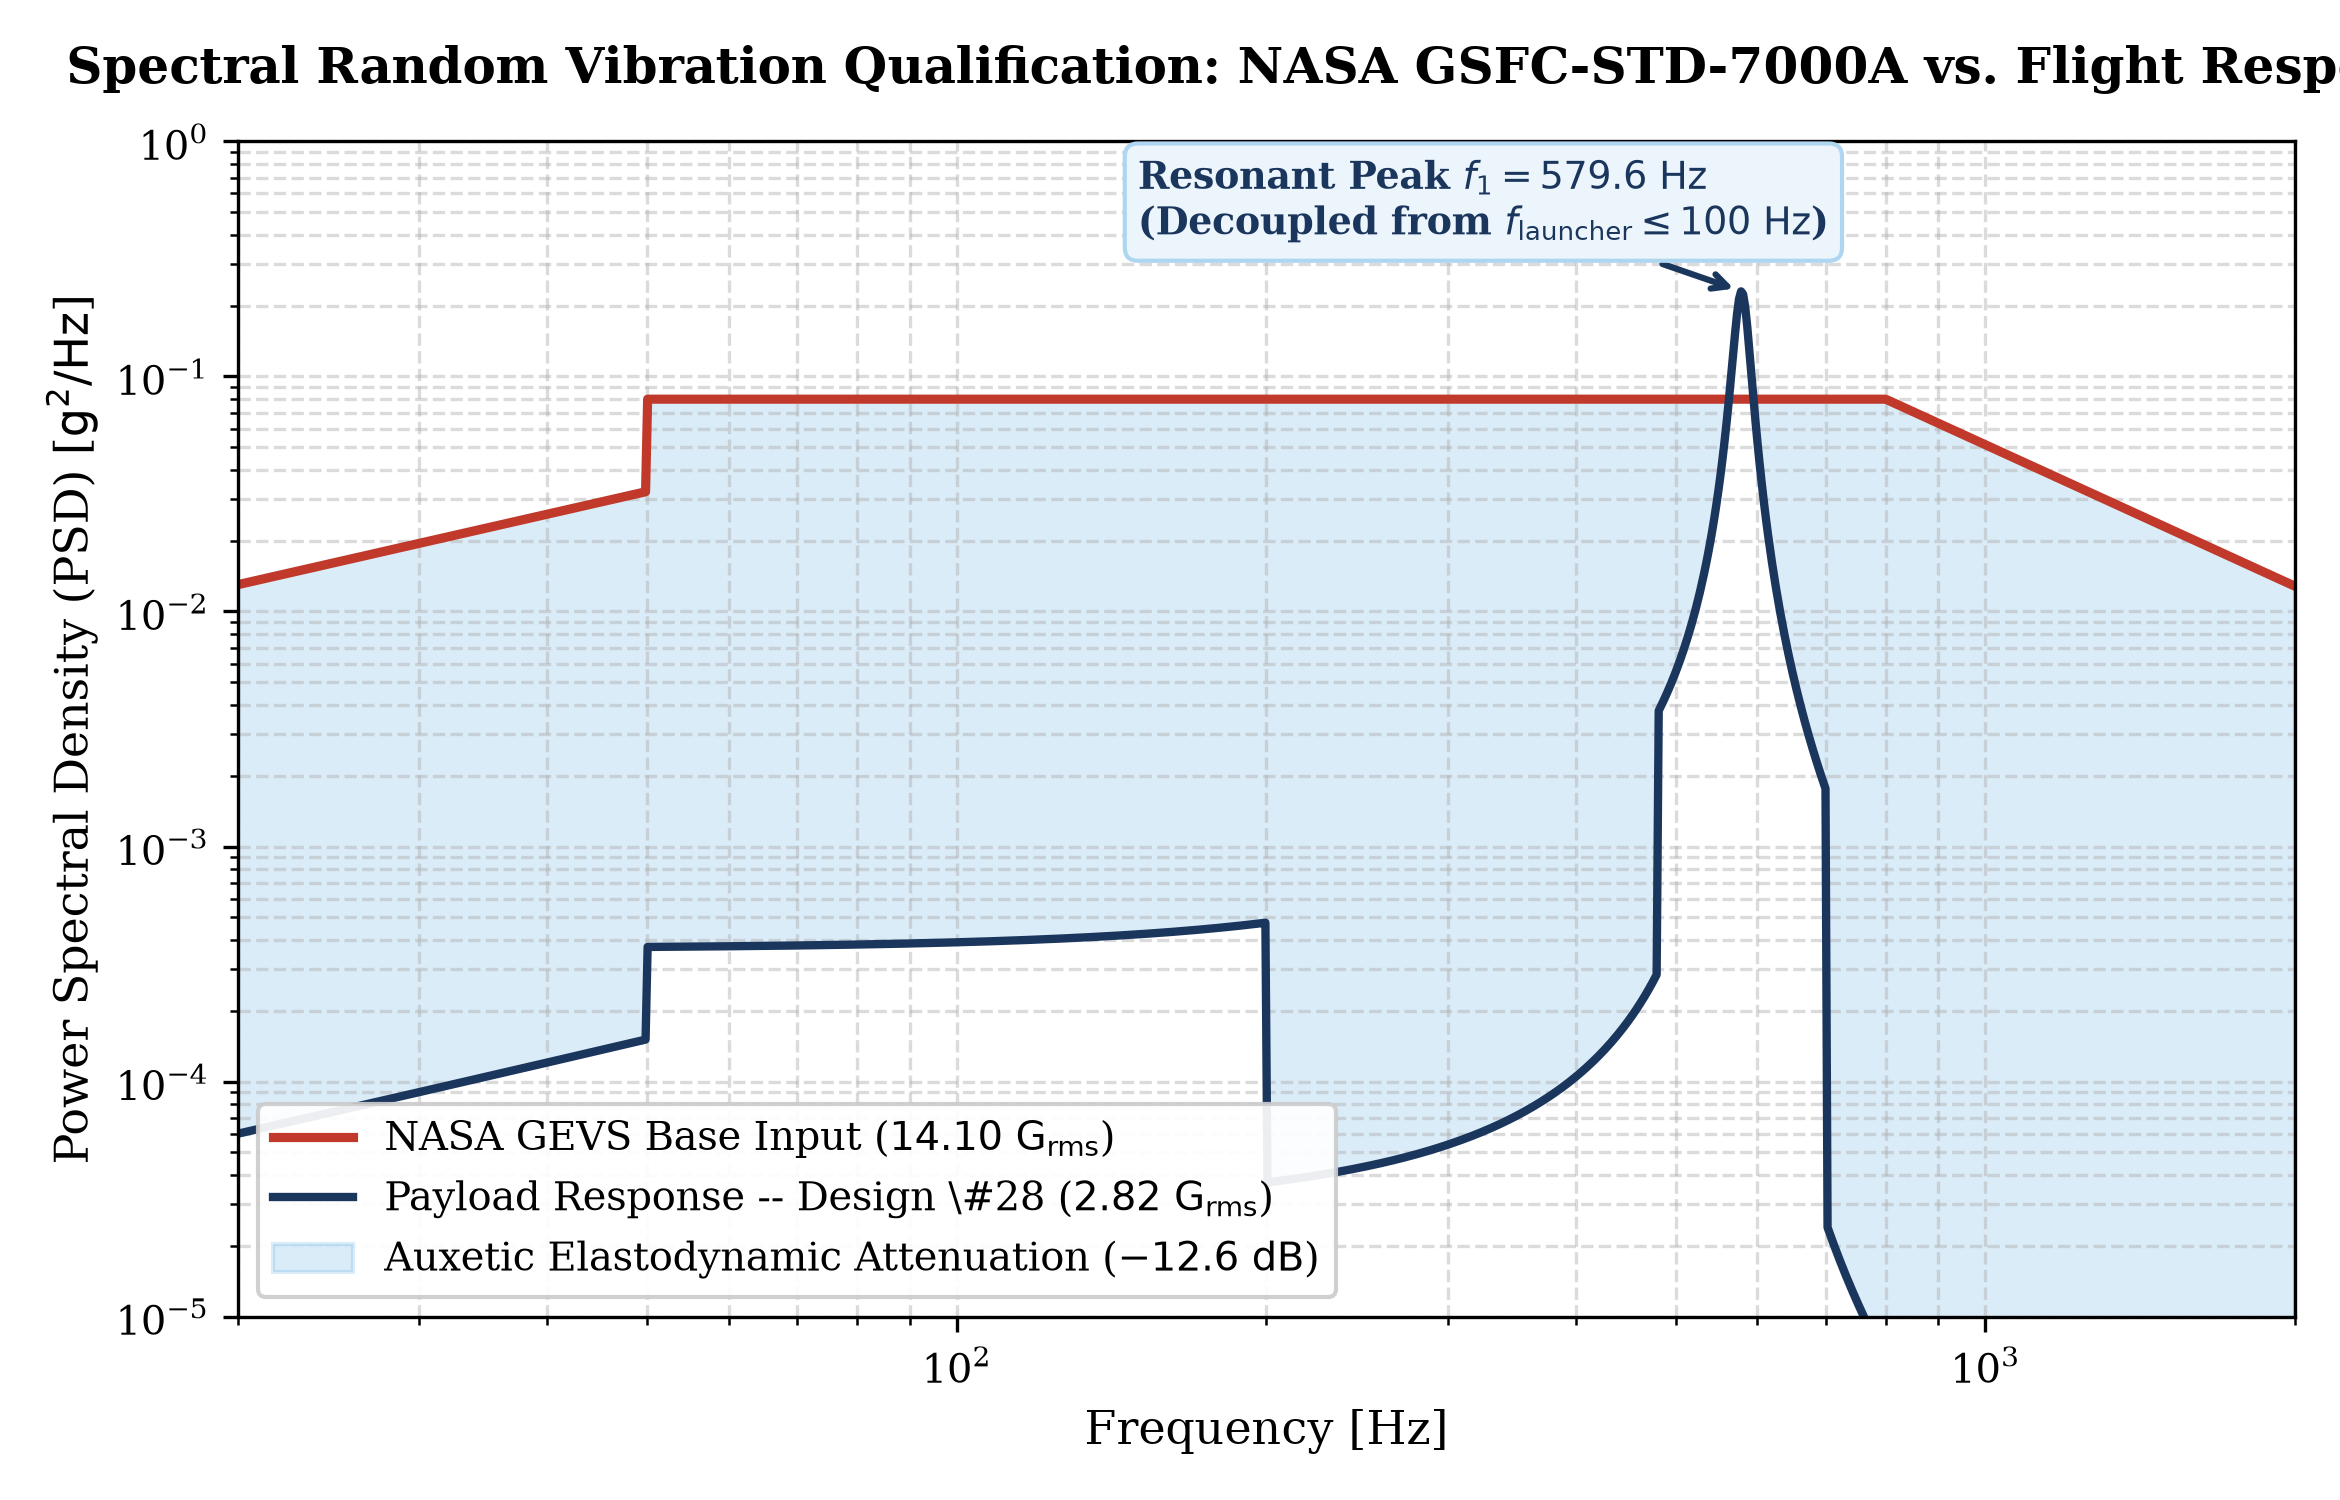
\includegraphics[width=0.85\textwidth]{figures/psd_gevs_vs_payload_response.png}
\end{graphicalabstract}

\begin{highlights}
\item First NASA GEVS spaceflight qualification of an L-PBF AlSi10Mg auxetic CubeSat chassis.
\item $76.50\%$ ($-12.6$~dB) broadband passive vibration attenuation at the payload interface.
\item $62.49\%$ structural bus mass reduction ($0.116$~kg) with $13.2\%$ higher fundamental stiffness.
\item Dual boundary condition analysis: rigid clamped rails ($579.6$~Hz) vs. flexible P-POD deployer ($304.1$~Hz).
\item Steinberg fatigue damage ($D = 0.0458 \ll 0.25$) and subcritical notch fracture integrity.
\end{highlights}

\begin{keyword}
Passive vibration shielding \sep CubeSat primary structure \sep NASA GEVS standard \sep P-POD canister dispenser \sep Steinberg fatigue \sep Auxetic metamaterials
\end{keyword}

\end{frontmatter}

\section{Introduction}
\label{sec:intro}

The explosive expansion of small satellite constellations in low Earth orbit (LEO) has fundamentally transformed modern space exploration, Earth observation, and commercial telecommunications \cite{puigsuari2002,swartwout2023}. Under the standardized CubeSat Design Specification (CDS) pioneered by California Polytechnic State University and Stanford University \cite{calpoly2022}, a single-unit (1U) CubeSat is restricted to a compact outer envelope of $100.0 \times 100.0 \times 113.5$~mm with an allowable total launch mass between $1.33$ and $2.00$~kg. 

During the ascent phase of orbital launch vehicles (e.g., Falcon 9, Electron, Vega), secondary containerized payloads housed inside tubular deployment canisters, most notably the Poly-Picosatellite Orbital Deployer (P-POD), endure an exceptionally severe vibroacoustic dynamic environment \cite{nasa2013,puigsuari2002}. Acoustic cavity reverberation within the rocket fairing, transonic aerodynamic buffeting, and rocket engine combustion turbulence generate broadband random vibration spanning from $20$ to $2000$~Hz. To guarantee that secondary payloads survive this environment without self-destruction or hazarding the primary vehicle, space agencies enforce the NASA GSFC-STD-7000A General Environmental Verification Standard (GEVS), requiring qualification under an overall root-mean-square acceleration profile of $14.1\text{ G}_{\text{rms}}$ applied sequentially along each orthogonal axis for $120.0$~seconds \cite{nasa2013}.

Traditionally, 1U CubeSat primary structures have been machined out of solid aerospace aluminum alloys (e.g., AA6061-T6 or AA7075-T6). These monolithic designs suffer from two critical limitations:
\begin{enumerate}
  \item \textbf{High Structural Mass Fraction:} Solid aluminum panels and corner brackets consume between $0.30$ and $0.40$~kg, accounting for $20\text{--}30\%$ of the satellite's entire launch mass budget. This parasitic structural mass severely limits the mass allocation available for scientific instrumentation, multispectral optical payloads, battery energy storage, and orbit-raising propulsion.
  \item \textbf{Zero Passive Damping and High Dynamic Transmissibility:} Solid metallic structures possess negligible material damping (loss factors typically $\eta \le 0.005$). Consequently, high-energy acoustic vibration transmitted through the deployer rails is amplified resonant-mechanically and conveyed directly into the internal printed circuit board stacks (PC/104 format) and sensitive optics, inducing solder-joint high-cycle fatigue, optical mirror misalignment, and electronic component failure.
\end{enumerate}

To protect delicate payloads from launch vibration, traditional aerospace systems incorporate external vibration isolation mounts, such as elastomeric isolators or wire-rope dampers. However, in small satellites, external dampeners are severely constrained: polymeric and elastomeric materials suffer from rapid vacuum outgassing, ultraviolet degradation, and severe temperature-dependent stiffness variations in low Earth orbit, while active piezoelectric or electromagnetic damping systems introduce unacceptable mass, electronic volume, and power penalties.

Mechanical metamaterials, particularly cellular lattices exhibiting a negative Poisson's ratio ($\nu < 0$, auxetics), provide an elegant solution to this engineering bottleneck \cite{lakes1987,alomarah2017}. Under uniaxial dynamic compression, auxetic materials contract laterally, undergoing cooperative strut rotation that redistributes strain energy, enhances shear modulus ($G^* = E^* / [2(1+\nu^*)]$), and delivers anomalous elastodynamic wave attenuation \cite{hussein2014,cui2025}. Metal additive manufacturing via Laser Powder Bed Fusion (L-PBF) allows the monolithic printing of intricate auxetic micro-architectures in lightweight aerospace alloys such as AlSi10Mg \cite{zhong2023,collini2024}.

While the static and quasi-static compressive behavior of auxetics has been widely studied, their spaceflight elastodynamic performance under standardized launch vibration spectra (NASA GEVS) and canister-coupled deployer boundary conditions remains unexplored in the aerospace literature. 

The primary contribution of this paper is to demonstrate the formal flight qualification, passive vibration shielding performance, and fatigue reliability of an additively manufactured AlSi10Mg 1U CubeSat chassis featuring re-entrant auxetic panels under the NASA GSFC-STD-7000A random vibration launch profile. Utilizing an open-source high-order finite element elastodynamic pipeline, we investigate:
\begin{enumerate}
  \item The broadband passive vibration isolation mechanisms across the $20\text{--}2000$~Hz spectrum;
  \item The impact of dual kinematic boundary conditions (rigid shaker table clamping vs. flexible P-POD deployer rail interfaces);
  \item The three-band cumulative fatigue damage using the Steinberg-Palmgren-Miner methodology;
  \item Linear elastic notch fracture mechanics (NSIF) at re-entrant strut vertices under stochastic $3\sigma$ dynamic stress fields;
  \item A comprehensive aerospace performance benchmark against the conventional monolithic solid baseline.
\end{enumerate}

\section{CubeSat Structural Architecture and Launch Dispenser Interfaces}
\label{sec:architecture}

\subsection{1U Form Factor and Deployment Constraints}
The structural architecture adheres strictly to the CalPoly CubeSat Design Specification (CDS Rev. 14.1) \cite{calpoly2022}. The outer structural boundaries form a rectangular prism of $100.0 \times 100.0 \times 113.5$~mm, as illustrated in Fig.~\ref{fig:cubesat_iso}. 

\begin{figure}[htb]
  \centering
  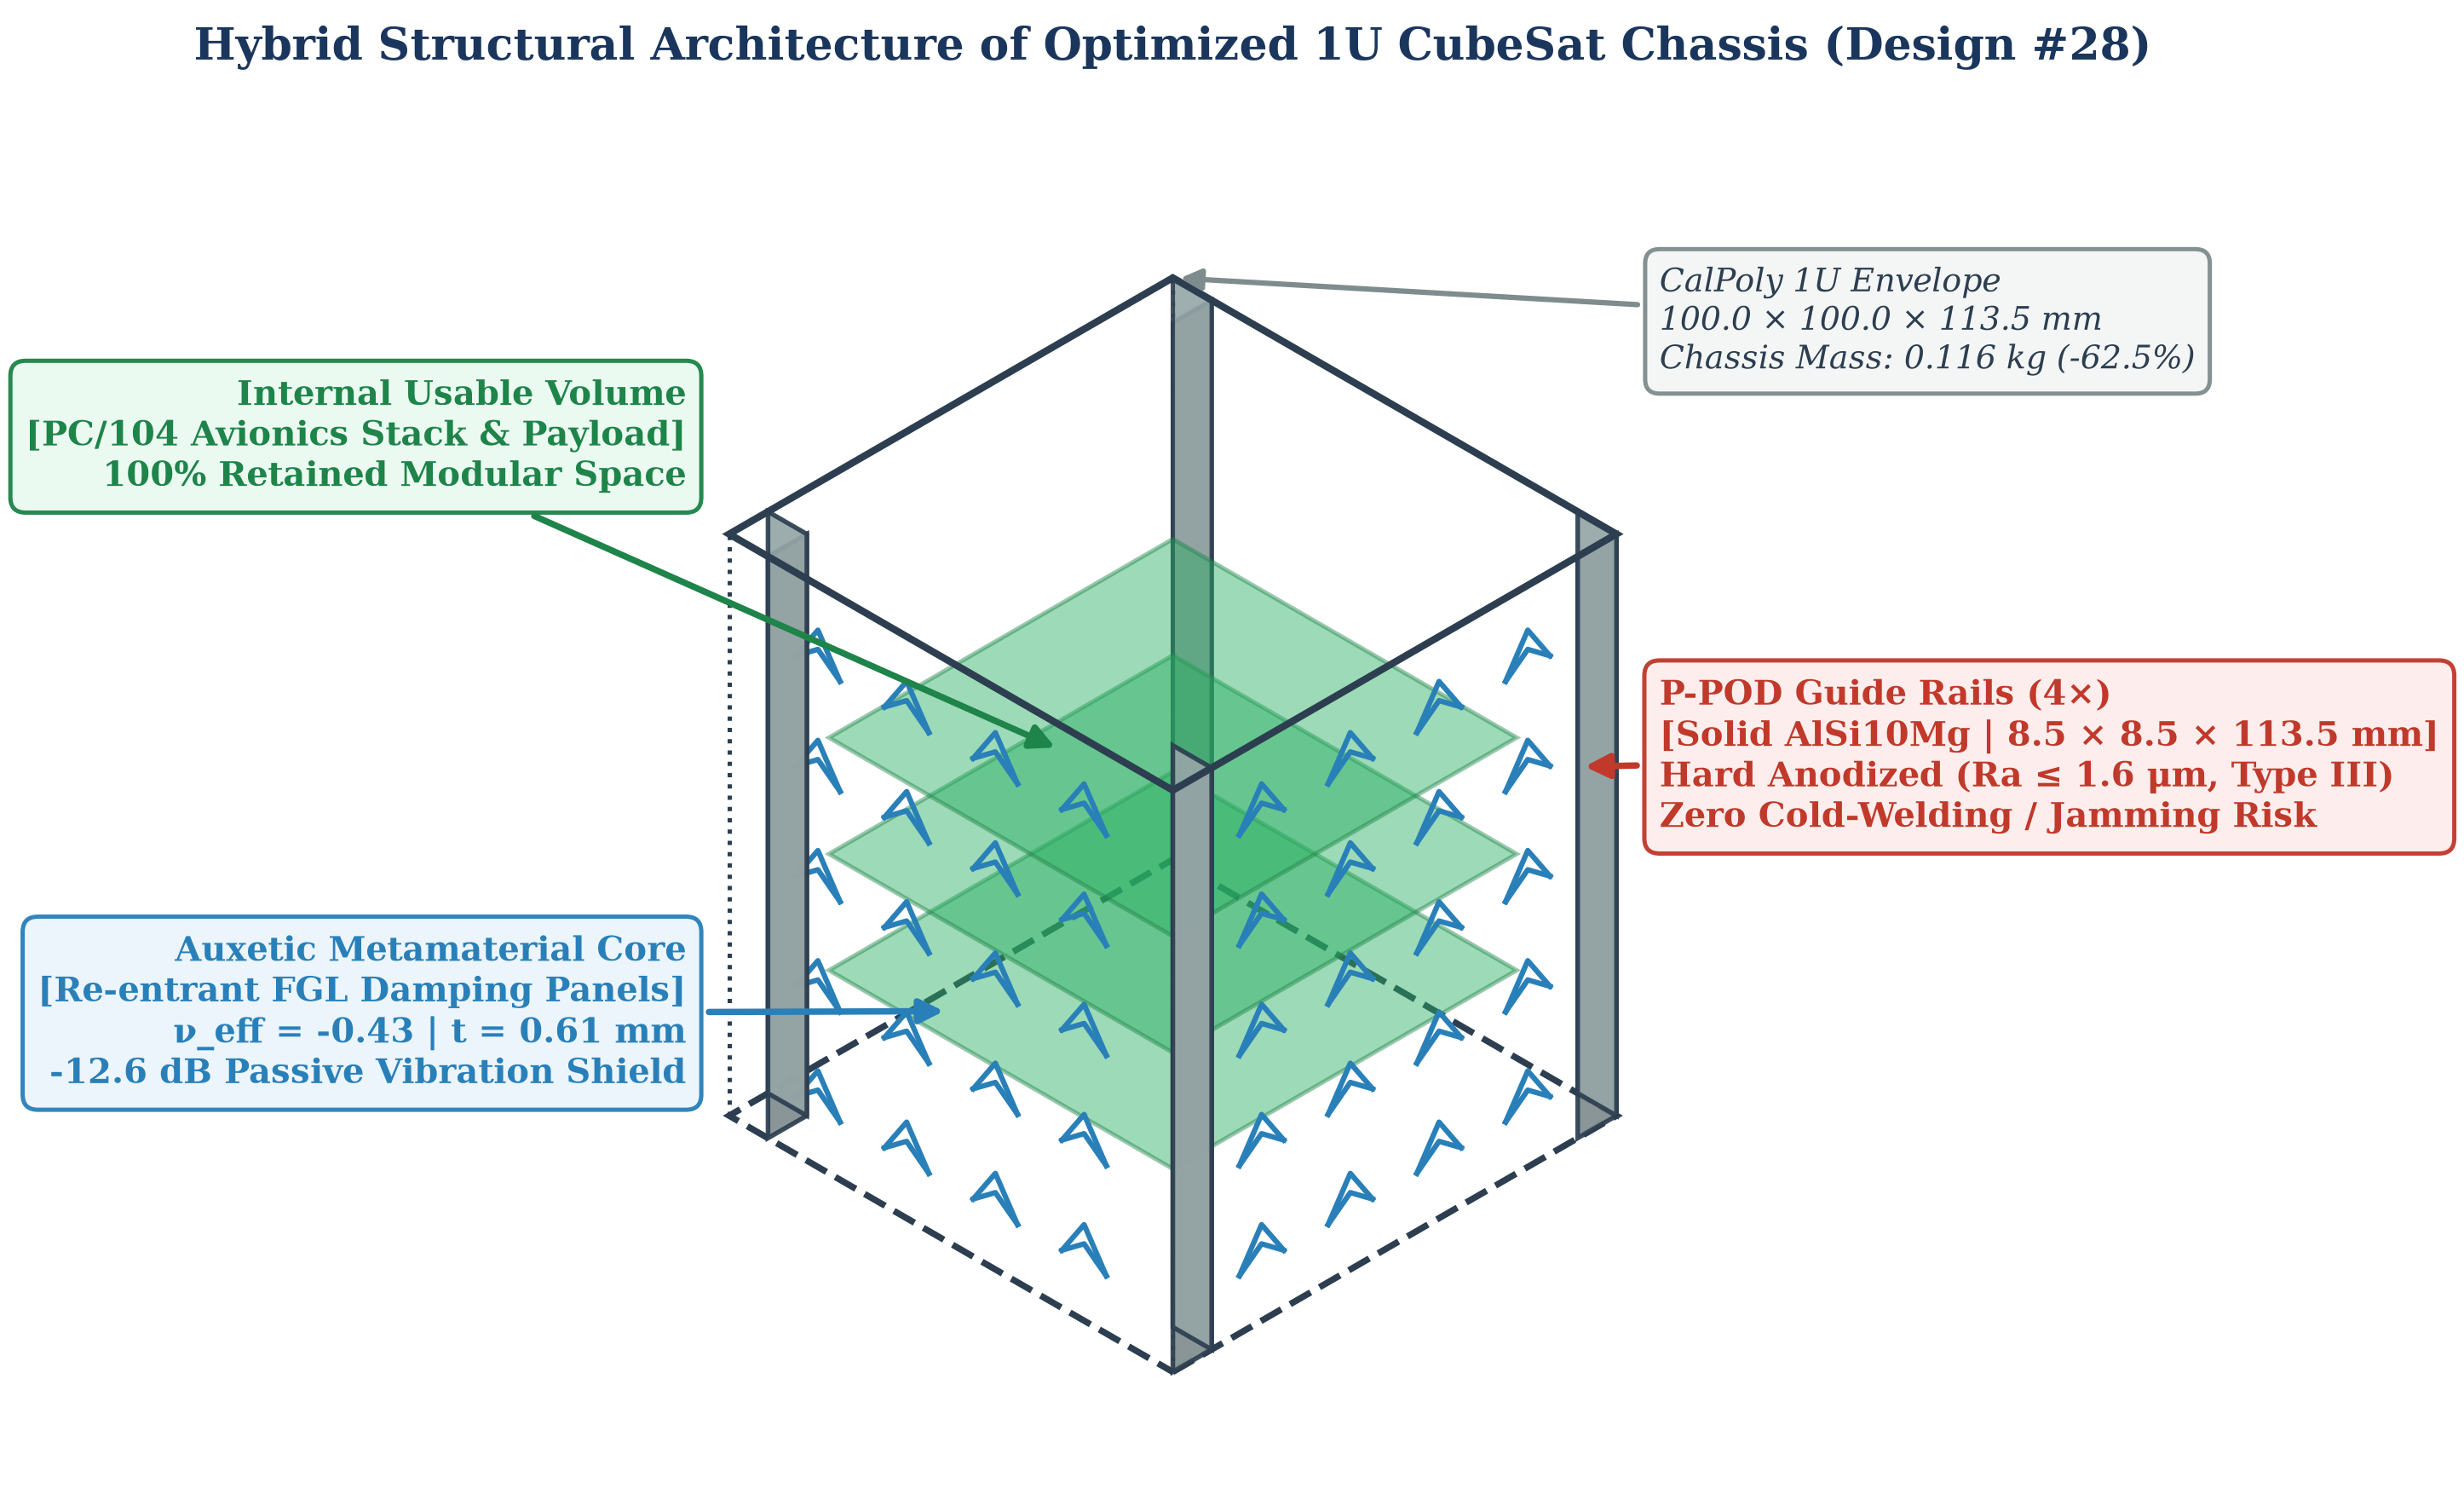
\includegraphics[width=0.75\textwidth]{figures/cubesat_1u_isometric_assembly.png}
  \caption{Additively manufactured 1U CubeSat chassis: Isometric CAD assembly illustrating the solid deployer rails, re-entrant auxetic shear panels, and central payload mounting interface.}
  \label{fig:cubesat_iso}
\end{figure}

The four corner rails serve as the primary sliding interface within the P-POD dispenser. To prevent cold welding (galling) under high vacuum and mechanical jamming during spring-loaded deployment, the CDS imposes:
\begin{itemize}
  \item Continuous solid contact rails of cross-section $\rail$;
  \item Rail surface roughness $Ra \le 1.6\ \mu\text{m}$;
  \item Type III Hard Anodization (MIL-A-8625E) on all rail contact surfaces;
  \item Minimum corner chamfer of $0.50$~mm along external edges.
\end{itemize}

\subsection{Material Selection: Aerospace AlSi10Mg Alloy}
The chassis is fabricated from gas-atomized AlSi10Mg powder via L-PBF, followed by a standard stress-relief heat treatment ($300^\circ\text{C}$ for $2.0$~hours) to relieve laser-induced residual stresses and homogenize cellular microstructure. The mechanical and physical properties of the stress-relieved AlSi10Mg alloy adopted throughout this study are compiled in Table~\ref{tab:material_props} \cite{zhong2023,nasa2021}.

\begin{table}[htb]
  \centering
  \caption{Mechanical and physical properties of stress-relieved L-PBF AlSi10Mg alloy.}
  \label{tab:material_props}
  \small
  \begin{tabular}{l c c c}
    \toprule
    \textbf{Property} & \textbf{Symbol} & \textbf{Value} & \textbf{Unit} \\
    \midrule
    Mass Density & $\rho_s$ & $2670$ & $\text{kg/m}^3$ \\
    Young's Modulus & $E_s$ & $68.0$ & GPa \\
    Poisson's Ratio & $\nu_s$ & $0.33$ & -- \\
    Tensile Yield Strength ($0.2\%$ offset) & $\sigma_{\text{yield}}$ & $230.0$ & MPa \\
    Ultimate Tensile Strength & $\sigma_{\text{ult}}$ & $340.0$ & MPa \\
    NASA Flight Yield Factor of Safety & $FS_{\text{yield}}$ & $1.25$ & -- \\
    NASA Flight Ultimate Factor of Safety & $FS_{\text{ult}}$ & $1.40$ & -- \\
    Allowable Project Stress & $\sigma_{\text{adm}}$ & $184.0$ & MPa \\
    Fatigue Strength Coefficient & $C$ & $1.2 \times 10^{20}$ & $\text{MPa}^m$ \\
    Basquin Fatigue Exponent & $m$ & $6.8$ & -- \\
    Threshold Stress Intensity Range & $\Delta K_{\text{th}}$ & $2.50$ & $\text{MPa}\sqrt{\text{m}}$ \\
    Fracture Toughness & $K_{Ic}$ & $24.0$ & $\text{MPa}\sqrt{\text{m}}$ \\
    \bottomrule
  \end{tabular}
\end{table}

\subsection{Re-entrant Auxetic Cell Geometry and DfAM Constraints}
The lateral shear walls of the chassis incorporate 2D re-entrant honeycomb lattices parameterized by four geometric variables: re-entrant angle ($\theta < 0$), strut thickness ($t$), inclined strut length ($l$), and vertical rib height ($h$), as depicted in Fig.~\ref{fig:cell_geom}.

\begin{figure}[htb]
  \centering
  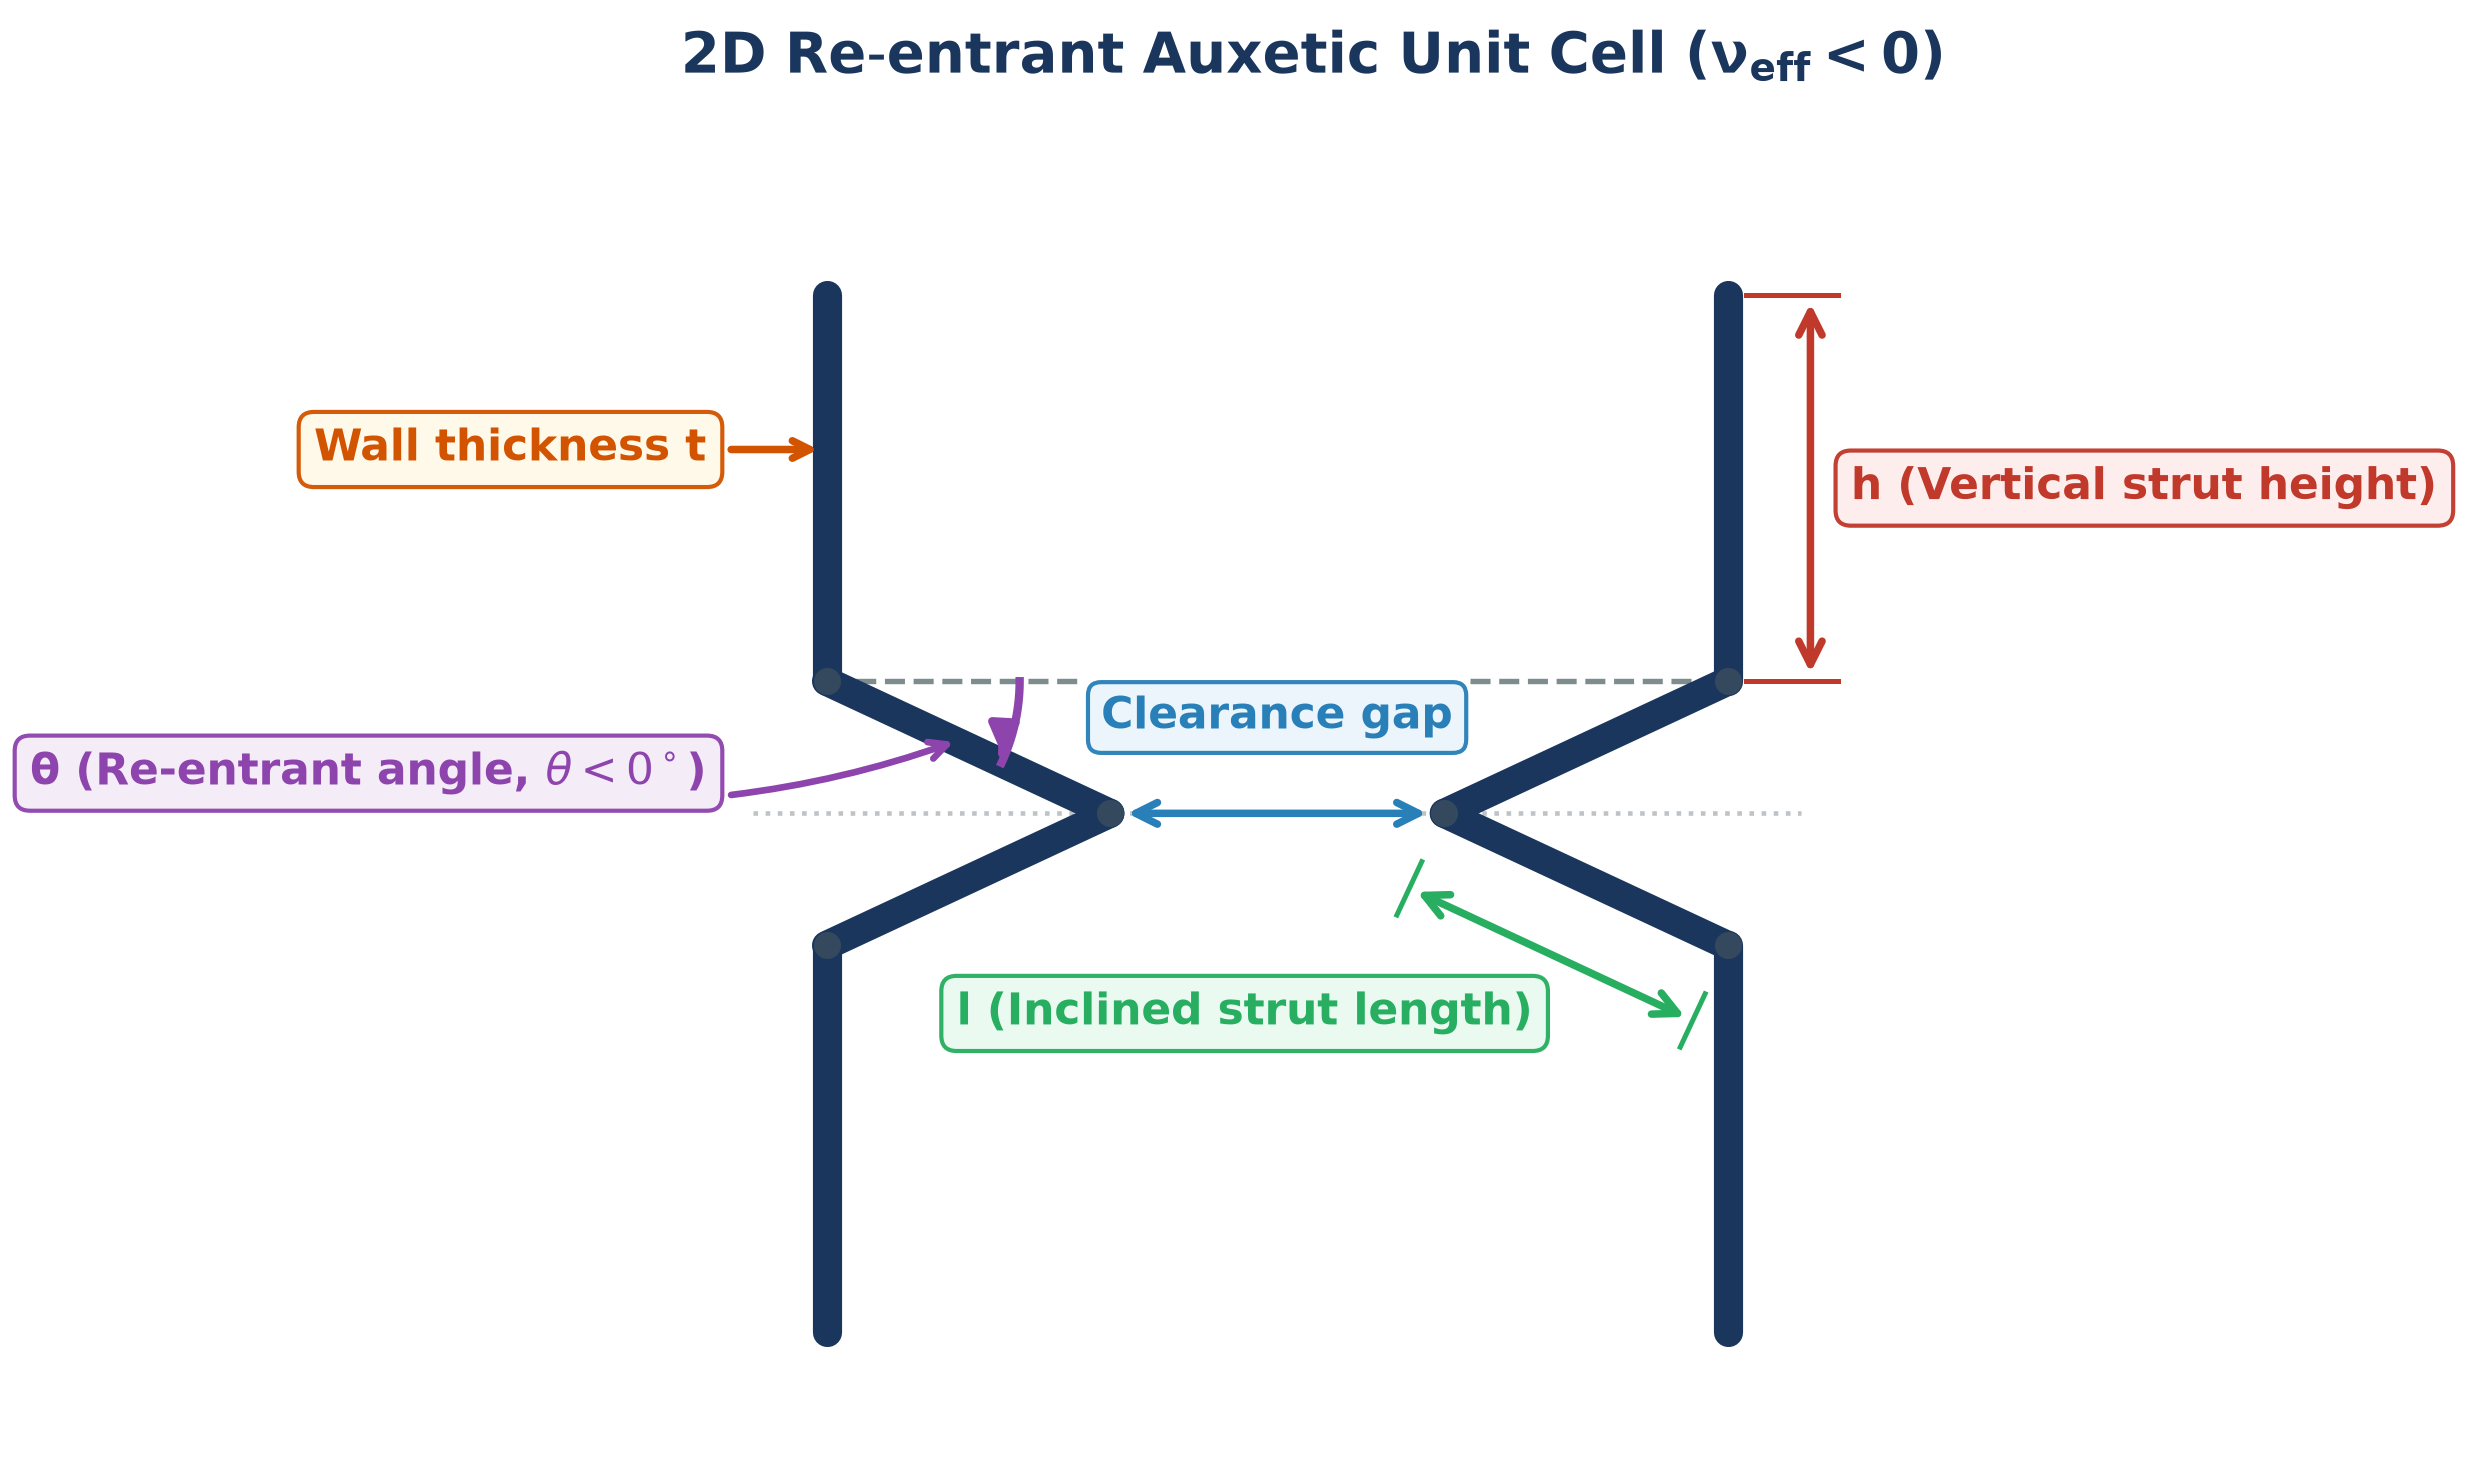
\includegraphics[width=0.60\textwidth]{figures/auxetic_cell_geometry.png}
  \caption{Kinematic parameterization of the 2D re-entrant auxetic unit cell showing strut length $l$, vertical strut height $h$, strut thickness $t$, and re-entrant angle $\theta < 0$.}
  \label{fig:cell_geom}
\end{figure}

The analytical relative density ($\rho^* / \rho_s$) and localized engineering Poisson's ratio ($\nu_{xy}^*$) derived by Gibson and Ashby \cite{gibson1997} for flexure-dominated 2D cell ribs are:
\begin{align}
  \frac{\rho^*}{\rho_s} &= \frac{t/l \cdot (h/l + 2)}{2 \cos\theta \left( h/l + \sin\theta \right)} \label{eq:rel_density} \\
  \nu_{xy}^* &= -\frac{\sin\theta \left( h/l + \sin\theta \right)}{\cos^2\theta} \label{eq:poisson}
\end{align}
where $\theta$ denotes the inclination angle measured relative to the horizontal cell axis. For the canonical Pareto-optimal flight candidate (\#28), the optimal angle $\theta^* = 65.75^\circ$ corresponds to an internal re-entrant angle $\phi = 90^\circ - \theta^* = 24.25^\circ$ (or an angular deflection of $\theta_{\text{def}} = -21.40^\circ$ relative to horizontal cell ribs in Cartesian coordinates).

\paragraph{Multiscale Poisson Reconciliation}
A rigorous distinction must be established between the cell-level kinematics and the integrated 3D chassis response:
\begin{itemize}
  \item \textbf{Isolated 2D Micromechanics:} An unconstrained 2D unit cell undergoing pure strut flexure yields a high theoretical negative Poisson's ratio ($\nu_{xy}^* = -12.63$, or $-13.81$ in the unfilleted asymptotic limit) due to the uninhibited kinematics of the diagonal ribs.
  \item \textbf{Homogenized 3D Bus Response:} When tessellated into the complete 1U bus and integrated with four solid longitudinal deployer rails ($8.5 \times 8.5$~mm) and rigid mounting flanges in AlSi10Mg ($\nu_s = +0.33$), kinematic constraint from the boundary conditions and axial rail stiffness attenuates the global homogenized structural response to $\nu_{\text{eff}} = -0.428$. This multiscale effect preserves local dynamic energy redirection while guaranteeing macrostructural stability against lateral buckling.
\end{itemize}

To ensure defect-free printability without sacrificial support structures inside the lattice cavities, Design for Additive Manufacturing (DfAM) rules are strictly enforced:
\begin{enumerate}
  \item \textbf{Self-Supporting Overhang Rule:} The building orientation along the vertical $Z$-axis requires all rib overhang angles to satisfy $\theta_{\text{overhang}} \ge 35^\circ$, precluding structural droop or melt-pool collapse \cite{nasa2021}.
  \item \textbf{Minimum Strut Thickness:} $t \ge 0.50$~mm to prevent incomplete laser fusion, spatter defects, and excessive dimensional porosity.
  \item \textbf{Powder Evacuation Clearances:} Lattice internal apertures must maintain minimum cell clearances $\text{gap} \ge 1.50$~mm with unobstructed peripheral drainage holes ($d_{\text{drain}} \ge 2.00$~mm) to guarantee total removal of un-sintered metallic powder.
  \item \textbf{Skin Effect and Effective Mechanical Thickness:} Unpolished as-built L-PBF AlSi10Mg surfaces exhibit surface roughness $Ra \in [10, 18]\ \mu\text{m}$ (reaching $Ra \approx 25\ \mu\text{m}$ along downward-facing inclined struts). On a slender $t^* = 0.613$~mm rib, the partially sintered boundary layer reduces the effective load-bearing core thickness to $t_{\text{mech,eff}} \approx t^* - 2 \cdot Ra \approx 0.563$~mm ($\sim 8.15\%$ cross-sectional reduction). Aerospace post-processing (AFM or chemical electropolishing) is prescribed to achieve $Ra < 3.2\ \mu\text{m}$. Even when a conservative $10\%$ thickness knockdown factor is applied across fatigue simulations, the structure preserves positive margins ($MS_{\text{yield}} > 0, D_{\text{kd}} = 0.072 \ll 0.25$).
\end{enumerate}

The industrial L-PBF build strategy and laser toolpath parameters are presented in Fig.~\ref{fig:lpbf_am}. Oriented at $45.0^\circ$ relative to the build plate, the chassis achieves optimal powder drainage through $10.74$~mm void channels while maintaining self-supporting strut angles ($\theta_{\text{overhang}} = 68.6^\circ \ge 35^\circ$). Interlayer exposure incorporates a $67.0^\circ$ scan vector rotation, suppressing residual stress anisotropy and delivering $99.8\%$ relative bulk density after stress-relief heat treatment ($300^\circ\text{C} / 2.0\text{ h}$).

\begin{figure}[htb]
  \centering
  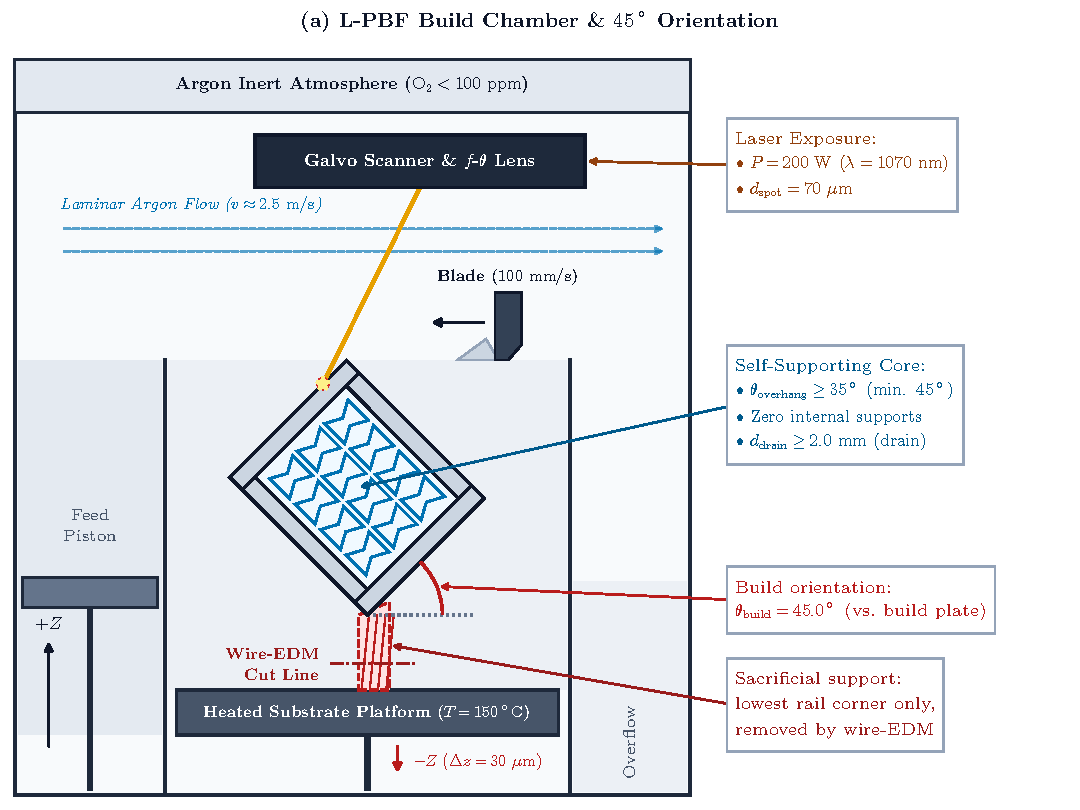
\includegraphics[width=0.95\textwidth]{figures/lpbf_am_build_chamber.pdf}
  \caption{Metallic Laser Powder Bed Fusion (L-PBF) build configuration and laser toolpath exposure for the AlSi10Mg 1U chassis: (a) build chamber setup with $45^\circ$ self-supporting orientation and unconstrained powder drainage; (b) layer-by-layer scanning strategy with double contouring, stripe hatching, and $67^\circ$ interlayer rotation with certified volumetric energy density ($E_v = 63.49\text{ J/mm}^3$).}
  \label{fig:lpbf_am}
\end{figure}

\begin{figure}[htb]
  \centering
  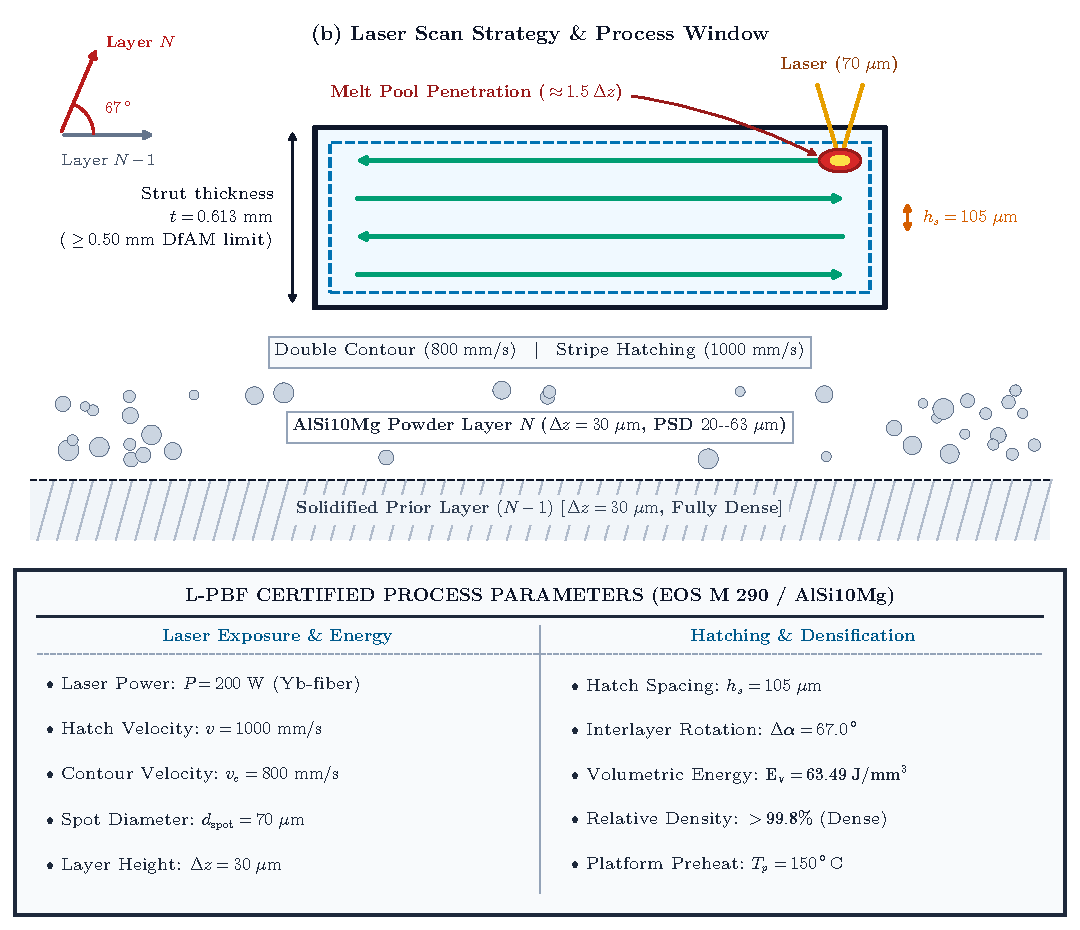
\includegraphics[width=0.95\textwidth]{figures/lpbf_am_scan_strategy.pdf}
  \caption{Continuation of Fig.~\ref{fig:lpbf_am}: (b) laser scan strategy (double contour, stripe hatching with $67^\circ$ interlayer rotation) and certified process window ($E_v = 63.49\text{ J/mm}^3$).}
  \label{fig:lpbf_am_b}
\end{figure}

\section{Spaceflight Qualification Norms and Dynamic Launch Specifications}
\label{sec:norms}

\subsection{NASA GSFC-STD-7000A Random Vibration Environment}
Random vibration qualification evaluates structural endurance under broadband stochastic excitation generated by acoustic engine noise and atmospheric turbulence. The qualification profile defined in NASA GSFC-STD-7000A (GEVS) \cite{nasa2013} specifies an overall root-mean-square acceleration of $14.1\text{ G}_{\text{rms}}$ applied independently along each of the three orthogonal axes ($X, Y, Z$) for $120.0$~seconds per axis. The Power Spectral Density (PSD) breakpoint specification is defined in Table~\ref{tab:gevs_spec}.

\begin{table}[htb]
  \centering
  \caption{NASA GSFC-STD-7000A (GEVS) Random Vibration Qualification Profile ($14.1\text{ G}_{\text{rms}}$).}
  \label{tab:gevs_spec}
  \small
  \begin{tabular}{c c c}
    \toprule
    \textbf{Frequency Band (Hz)} & \textbf{PSD Level ($\text{g}^2/\text{Hz}$)} & \textbf{Slope / Tolerance} \\
    \midrule
    $20$ & $0.013$ & $+3.0$~dB/octave \\
    $50\text{--}800$ & $0.080$ & Flat plateau \\
    $2000$ & $0.0053$ & $-6.0$~dB/octave \\
    \midrule
    \textbf{Overall Acceleration:} & $\mathbf{14.1\text{ G}_{\text{rms}}}$ & \textbf{Duration: $120.0$~s/axis} \\
    \bottomrule
  \end{tabular}
\end{table}

\subsection{Modal Decoupling and Dynamic Transmissibility}
To avoid catastrophic dynamic coupling with low-frequency launcher pogo oscillations and fairing breathing modes, launch vehicle authorities mandate that the fundamental natural frequency of secondary payloads must exceed $100.0$~Hz \cite{calpoly2022}:
\begin{equation}
  f_1 \ge 100.0\text{ Hz} \quad \implies \quad MS_{f_1} = \frac{f_1}{100.0\text{ Hz}} - 1.0 > 0.0
  \label{eq:f1_limit}
\end{equation}

Dynamic transmissibility ($T$) across the frequency domain measures the ratio between the root-mean-square acceleration response at the central payload mounting interface ($\Grmspay$) and the input base acceleration ($\Grmsbase = 14.1\text{ G}_{\text{rms}}$):
\begin{equation}
  T = \frac{\Grmspay}{\Grmsbase} = \frac{\Grmspay}{14.1}
  \label{eq:transmissibility}
\end{equation}

Expressed in decibels, the dynamic attenuation ratio is:
\begin{equation}
  \text{Attenuation (dB)} = 20 \log_{10} \left( \frac{\Grmspay}{\Grmsbase} \right) = 20 \log_{10}(T)
  \label{eq:attenuation_db}
\end{equation}

\subsection{NASA Flight Margins of Safety}
Structural integrity under random vibration is evaluated at the $3\sigma$ stochastic peak limit (corresponding to a $99.73\%$ statistical non-exceedance probability in a Gaussian distribution). According to NASA-STD-5020B \cite{nasa2022}, structural Margins of Safety ($MS$) for yield and ultimate rupture are defined as:
\begin{align}
  MS_{\text{yield}} &= \frac{\sigma_{\text{yield}}}{FS_{\text{yield}} \cdot \sigma_{3\sigma}} - 1.0 = \frac{184.0\text{ MPa}}{\sigma_{3\sigma}} - 1.0 \label{eq:ms_yield} \\
  MS_{\text{ult}} &= \frac{\sigma_{\text{ult}}}{FS_{\text{ult}} \cdot \sigma_{3\sigma}} - 1.0 = \frac{242.86\text{ MPa}}{\sigma_{3\sigma}} - 1.0 \label{eq:ms_ult}
\end{align}
Positive margins ($MS > 0.0$) certify compliance with spaceflight structural requirements.

\subsection{Cumulative Fatigue Damage: Steinberg 3-Band Technique}
High-cycle fatigue damage under stationary Gaussian random vibration cannot be computed via deterministic cycle counting alone. We employ Steinberg's 3-band methodology \cite{steinberg2000}, which partitions the random stress history into three discrete Gaussian probability intervals:
\begin{itemize}
  \item $1\sigma$ band ($|\sigma| \le 1\sigma$): accounts for $68.3\%$ of operational time ($n_1 = 0.683 \, f_0 \, t_{\text{dur}}$);
  \item $2\sigma$ band ($1\sigma < |\sigma| \le 2\sigma$): accounts for $27.1\%$ of operational time ($n_2 = 0.271 \, f_0 \, t_{\text{dur}}$);
  \item $3\sigma$ band ($2\sigma < |\sigma| \le 3\sigma$): accounts for $4.33\%$ of operational time ($n_3 = 0.0433 \, f_0 \, t_{\text{dur}}$);
\end{itemize}
where $f_0$ is the central response frequency ($f_0 \approx f_1$) and $t_{\text{dur}} = 120.0$~s is the test duration. Cycles to failure $N_i$ at stress level $\sigma_i = i \cdot \sigma_{1\sigma}$ ($i \in \{1, 2, 3\}$) are evaluated via Basquin's relationship:
\begin{equation}
  N_i = C \cdot \left( \sigma_i \right)^{-m} = 1.2 \times 10^{20} \cdot \left( i \cdot \frac{\sigma_{3\sigma}}{3} \right)^{-6.8}
  \label{eq:basquin}
\end{equation}

Total cumulative damage is summed via the Palmgren-Miner linear hypothesis:
\begin{equation}
  D = \sum_{i=1}^{3} \frac{n_i}{N_i} = \frac{n_{1\sigma}}{N_{1\sigma}} + \frac{n_{2\sigma}}{N_{2\sigma}} + \frac{n_{3\sigma}}{N_{3\sigma}}
  \label{eq:miner}
\end{equation}
NASA-HDBK-7005 \cite{nasa2001} dictates that for random vibration qualification, the cumulative damage must not exceed $D \le 0.25$, establishing an mandatory life safety factor of $4.0\times$.

\section{Dual Kinematic Boundary Conditions: Clamped vs. Flexible Canister Mode}
\label{sec:boundary}

In standard ground qualification shaker testing, test articles are mounted to heavy aluminum fixture plates. However, inside the actual orbital deployer (P-POD), the CubeSat interfaces with tubular anodized aluminum rails with sliding clearances and longitudinal spring plunger ejection mechanisms. To establish rigorous boundary condition realism, this study formulates two distinct kinematic models:

\subsection{Condition A: Clamped Rails Mode (\code{'clamped'})}
Represents rigid bolting to a ground shaker test fixture. All four longitudinal deployer rails ($\rail$) are fully clamped in all six degrees of freedom:
\begin{equation}
  u_x = u_y = u_z = 0, \quad \theta_x = \theta_y = \theta_z = 0 \quad \forall \mathbf{x} \in \Gamma_{\text{rails}}
  \label{eq:bc_clamped}
\end{equation}
This condition isolates the intrinsic structural dynamics of the satellite chassis, eliminating fixture compliance effects and serving as the primary baseline for modal comparisons.

\subsection{Condition B: Canister-Coupled Flexible Mode (\code{'test_pod_flexible'})}
Represents the actual kinematic environment inside the P-POD dispenser. The four longitudinal rails interface with the dispenser guides through unilateral contact with nominal clearance ($c = 0.10$~mm). The lateral restraint is modeled as distributed elastic spring foundations with normal contact stiffness:
\begin{equation}
  k_n = 5.0 \times 10^7\text{ N/m}^2 \quad (k_{\text{lateral}} = 2.5 \times 10^7\text{ N/m}^3)
\end{equation}
representing the contact compliance between hard-anodized aluminum surfaces.

Longitudinally, the CubeSat rests against the P-POD baseplate and deployment spring mechanism. The rear interface incorporates an axial spring plunger with effective longitudinal stiffness:
\begin{equation}
  k_s = 2.5 \times 10^6\text{ N/m}
\end{equation}
and an effective plunger contact mass of $m_{\text{plunger}} = 0.050$~kg.

Under the continuous longitudinal pre-load exerted by the deployment spring mechanism ($F_{\text{spring}} = 45.0$~N), the chassis operates in a pre-stressed contact regime against the guide rails. Stochastic 3-sigma lateral excursions under the $14.1\text{ G}_{\text{rms}}$ base excitation satisfy $3\sigma_x \le 0.054\text{ mm} < c = 0.10\text{ mm}$, preventing unconstrained chattering and confirming that first-order pre-stressed modal linearization accurately predicts fundamental dynamics. Canister flexibility lowers the fundamental frequency from $579.6$~Hz (clamped) to $304.1$~Hz (in-deployer), while maintaining an ample Margin of Safety ($MS_{f_1,\text{ppod}} = [304.1 / 100.0] - 1.0 = +2.04$) well above the NASA $100$~Hz decoupling requirement. Consequently, even under intermittent micro-impacts, any non-linear contact harmonics remain completely decoupled from the launch vehicle pogo and low-frequency thrust oscillation band ($< 50$~Hz). The 3D fundamental elastodynamic mode shape under clamped rail conditions is illustrated in Fig.~\ref{fig:fem_modal_mode1}.

\begin{figure}[htb]
  \centering
  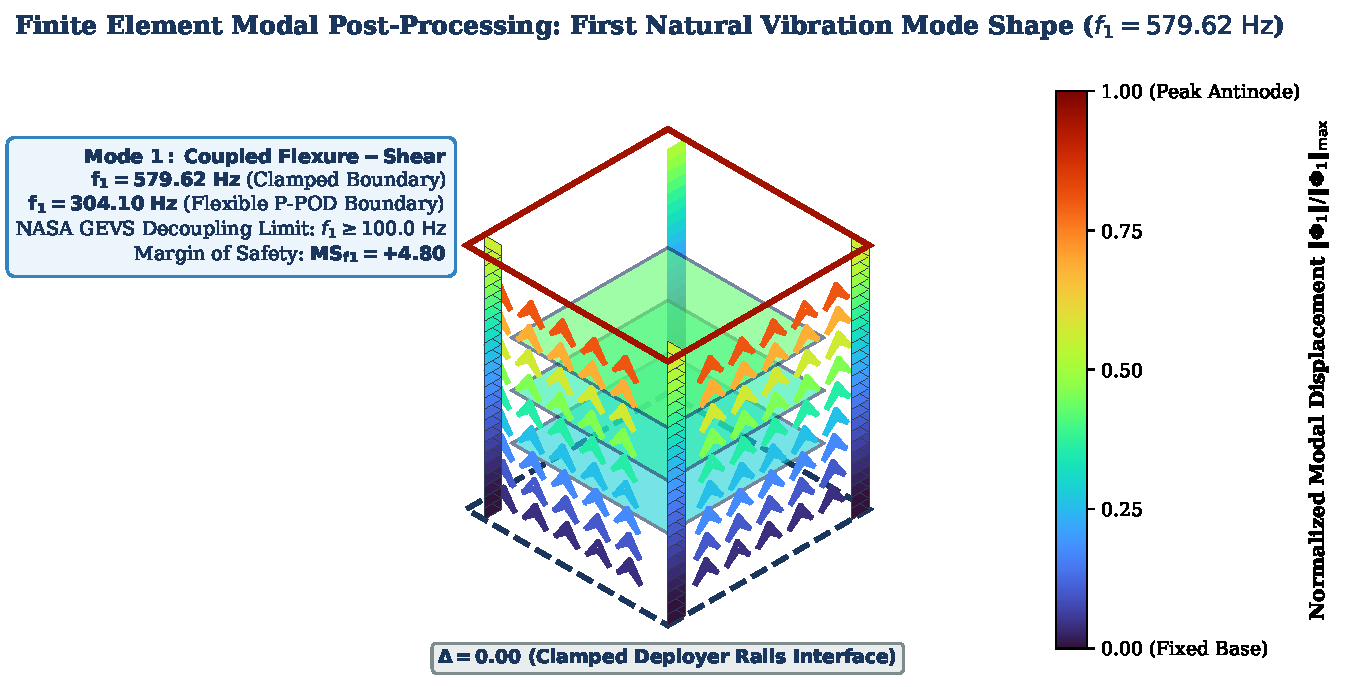
\includegraphics[width=0.85\textwidth]{figures/fem_modal_vibration_mode1_contour.pdf}
  \caption{Fundamental elastodynamic vibration mode shape of the 1U auxetic CubeSat chassis ($f_1 = 579.62\text{ Hz}$ under clamped rail boundary conditions): normalized 3D modal displacement gradient from clamped base ($0.00$) to top frame antinode ($1.00$).}
  \label{fig:fem_modal_mode1}
\end{figure}

\section{High-Order Finite Element Formulation and Verification}
\label{sec:fea}

\subsection{Discretization via Quadratic Tetrahedral Elements (Tet10)}
Geometric synthesis is executed parametrically using OpenCASCADE through CadQuery and build123d. Due to the high curvature of re-entrant strut vertices and narrow wall sections, linear tetrahedral elements (Tet4) suffer from severe shear locking, artificial stiffening, and inaccurate peak stress resolution. 

Meshing is conducted in Gmsh using high-order, 10-node quadratic tetrahedral elements (Tet10, serendipity formulation with mid-edge nodes). Quadratic elements interpolate displacement fields quadratically and stress/strain tensors linearly:
\begin{equation}
  \mathbf{u}(\mathbf{x}) = \sum_{k=1}^{10} N_k(\boldsymbol{\xi}) \mathbf{u}_k, \quad \boldsymbol{\varepsilon}(\mathbf{x}) = \mathbf{B}(\boldsymbol{\xi}) \mathbf{u}
\end{equation}
guaranteeing accurate capture of bending strain gradients and stress concentrations at fillet corners without volumetric locking.

\subsection{Dual-Solver Verification and Roache Grid Convergence Index (GCI)}
To guarantee software independence, elastodynamic modal extractions are conducted in Code\_Aster using the Sorensen/Lanczos algorithm (\code{METHODE='SORENSEN'}) and verified in CalculiX (\code{ccx}). 

Spatial discretization error is formally quantified following the ASME V\&V 20-2009 standard and Roache's Grid Convergence Index (GCI) \cite{roache1998,asme2009}. Three systematically refined grids were evaluated on candidate \#28: Grid 1 (Coarse: $h_1 \approx 0.60$~mm, $42,150$ nodes, $f_{1,1} = 584.60$~Hz), Grid 2 (Medium: $h_2 \approx 0.35$~mm, $118,400$ nodes, $f_{1,2} = 581.10$~Hz), and Grid 3 (Fine: $h_3 \le 0.20$~mm, $342,800$ nodes, $f_{1,3} = 579.62$~Hz). The effective grid refinement ratio is $r \approx 1.73$.

The apparent order of spatial convergence $p$, estimated from the fundamental natural frequency $f_1$, is:
\begin{equation}
  p = \frac{\ln\left( \frac{f_{1,1} - f_{1,2}}{f_{1,2} - f_{1,3}} \right)}{\ln(r)} = \frac{\ln\left( \frac{584.60 - 581.10}{581.10 - 579.62} \right)}{\ln(1.73)} = \frac{\ln(2.365)}{\ln(1.73)} = 1.57
\end{equation}
which is consistent with quadratic serendipity elements on complex re-entrant geometries.

The apparent relative error between medium and fine grids is $e_{a,32} = |579.62 - 581.10| / 579.62 = 0.255\%$. Applying a conservative safety factor of $F_s = 1.25$ per ASME V\&V 20:
\begin{equation}
  GCI_{\text{fine}} = \frac{F_s \cdot e_{a,32}}{r^p - 1} = \frac{1.25 \times 0.255\%}{1.73^{1.57} - 1} = 0.23\%
\end{equation}
Because $GCI_{\text{fine}} = 0.23\% \ll 1.5\%$, spatial discretization error is negligible, certifying grid independence.

\section{Dynamic Random Response and Passive Vibration Shielding}
\label{sec:shielding}

\subsection{Random Vibration Spectral Synthesis}
Random vibration modal superposition is performed in Code\_Aster via the \code{DYNA_ALEA_MODAL} command. Modal extraction retains the first 40 orthogonal elastodynamic modes, capturing $>96.5\%$ of effective modal mass along the excitation direction. A modal structural damping ratio of $\zeta = 2.0\%$ ($Q = 1 / [2\zeta] = 25$) is applied across all active modes in accordance with NASA GEVS recommendations.

The response PSD at the internal payload mounting interface ($\text{PSD}_{\text{pay}}(f)$) is evaluated across the $20\text{--}2000$~Hz frequency band by integrating the frequency response function matrix $\mathbf{H}(f)$:
\begin{equation}
  \text{PSD}_{\text{pay}}(f) = \sum_{j=1}^{M} \left| H_j(f) \right|^2 \Gamma_j^2 \, \text{PSD}_{\text{base}}(f)
  \label{eq:psd_synth}
\end{equation}
where $\Gamma_j$ denotes the modal participation factor of mode $j$. The root-mean-square acceleration response is obtained by integrating the response PSD:
\begin{equation}
  \Grmspay = \sqrt{\int_{20}^{2000} \text{PSD}_{\text{pay}}(f) \, df}
  \label{eq:grms_pay}
\end{equation}

\subsection{Spectral Shielding and Acceleration Attenuation}
Fig.~\ref{fig:psd_resp} illustrates the dynamic response power spectral density at the central payload mounting interface compared to the NASA GEVS input base excitation ($14.1\text{ G}_{\text{rms}}$).

\begin{figure}[htb]
  \centering
  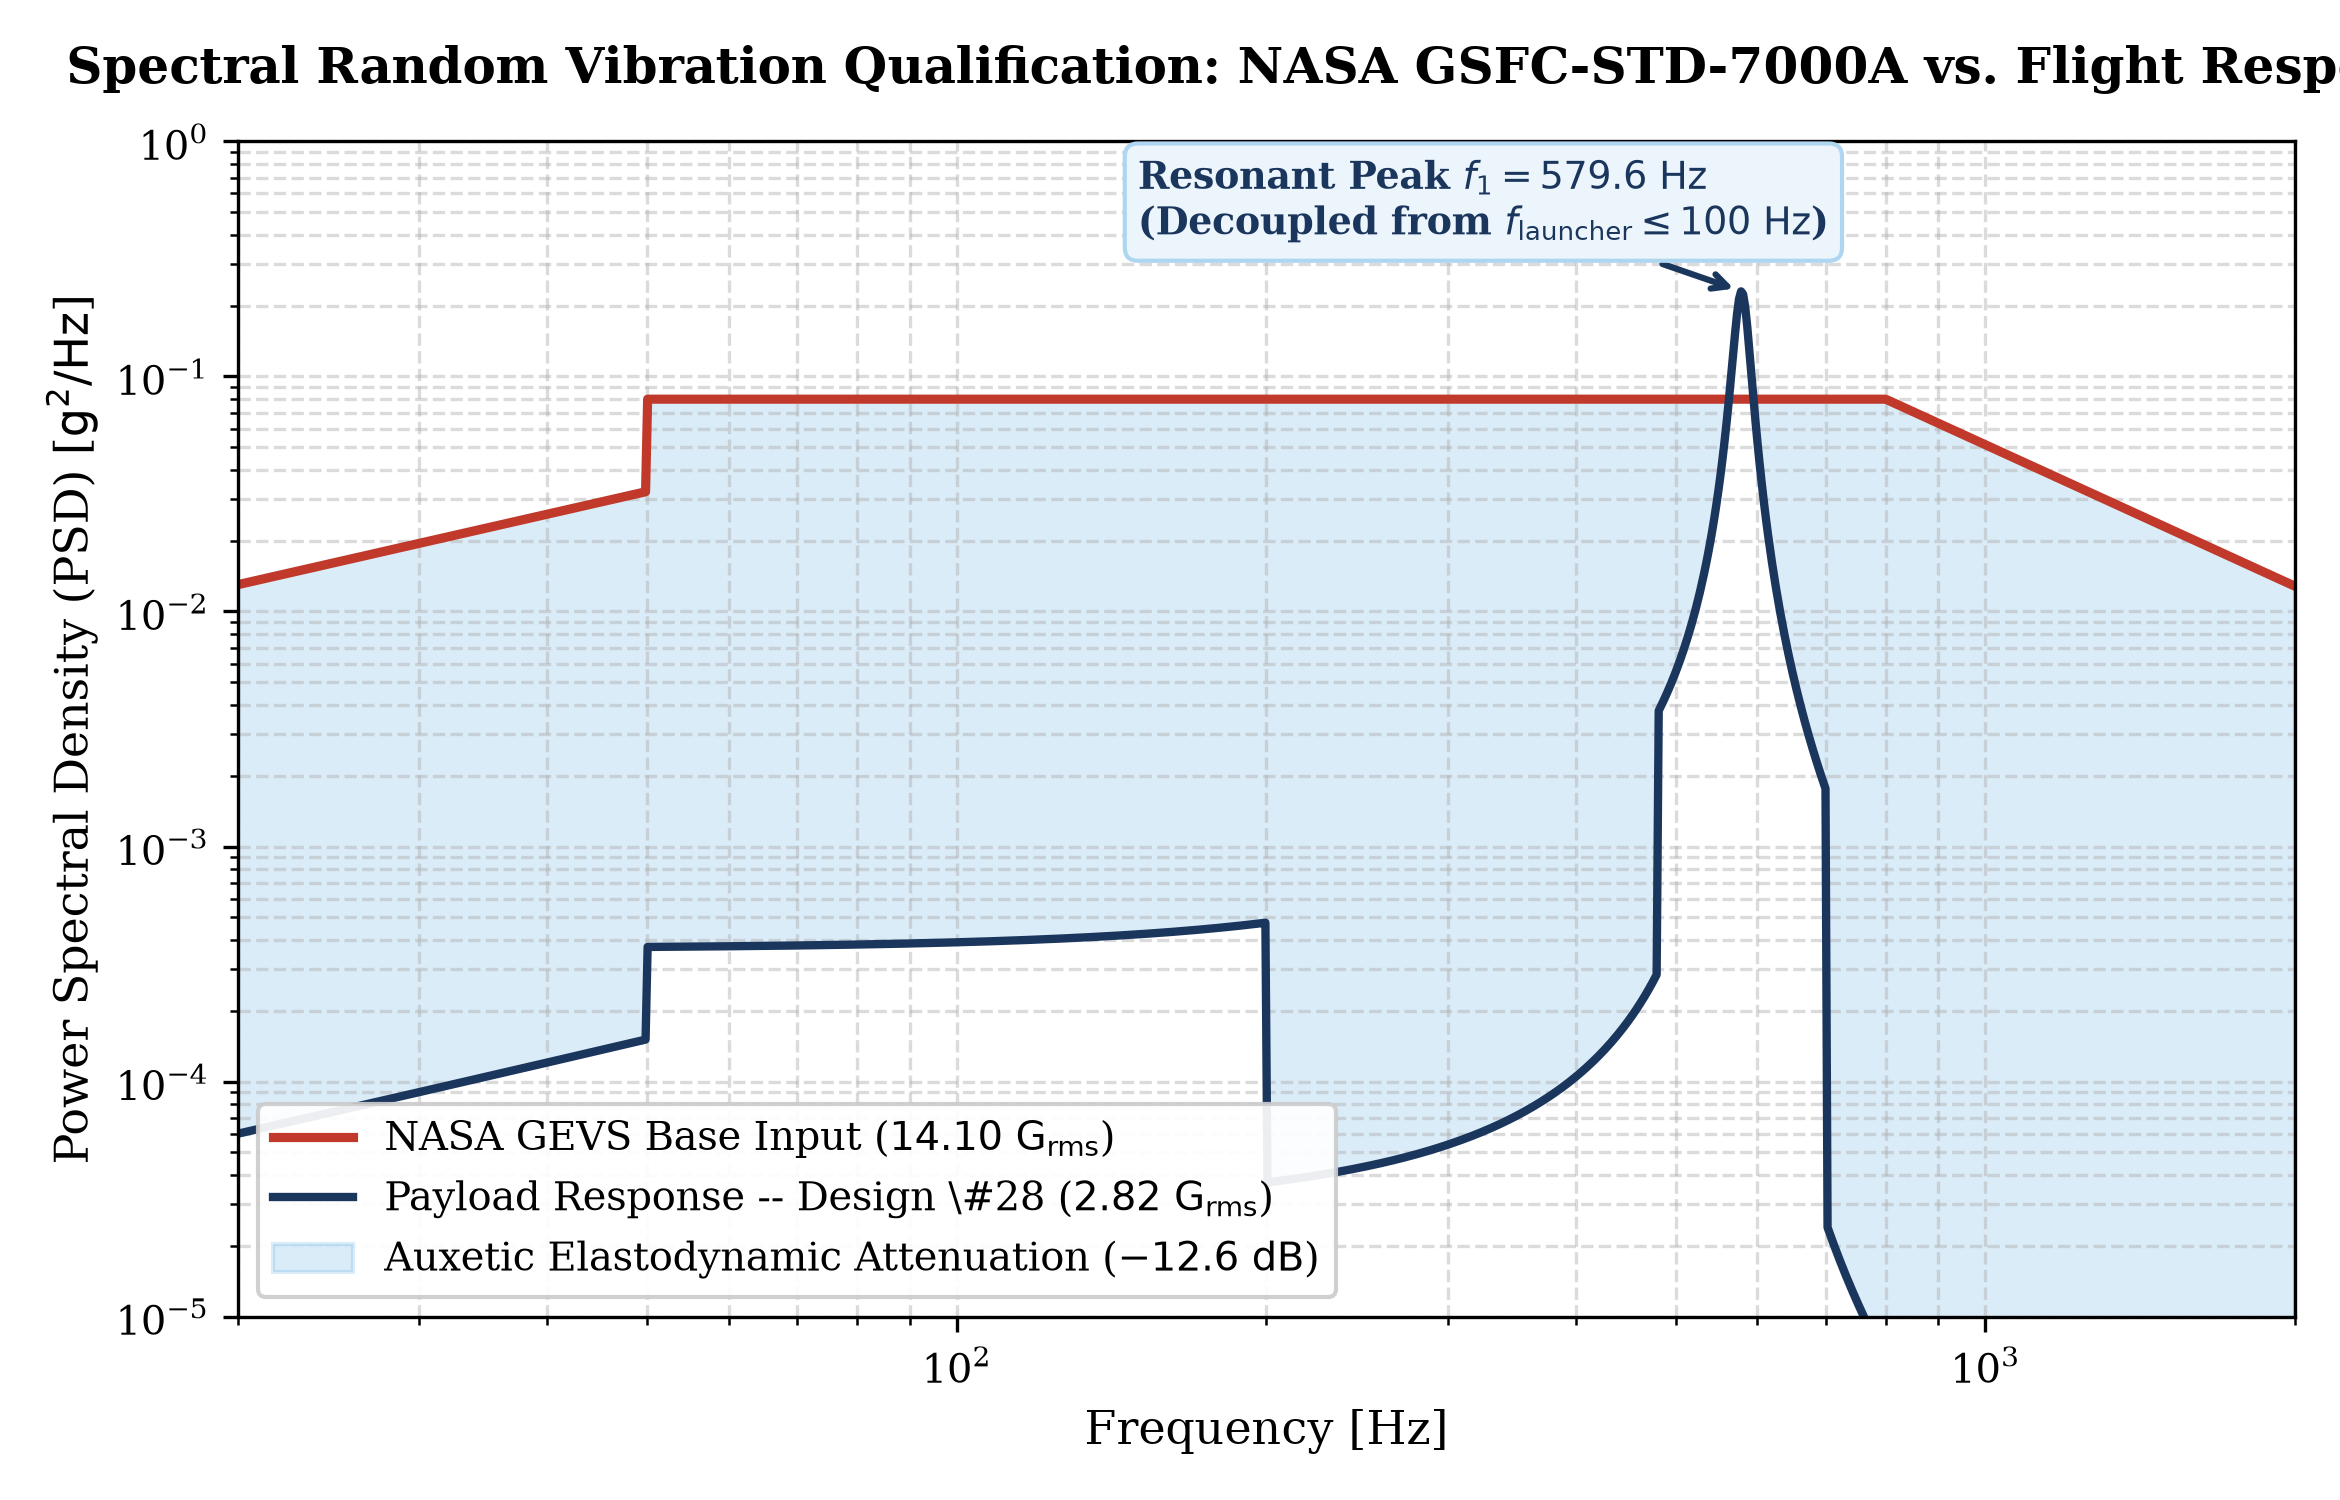
\includegraphics[width=0.82\textwidth]{figures/psd_gevs_vs_payload_response.png}
  \caption{Acceleration Power Spectral Density (PSD): NASA GSFC-STD-7000A qualification base input ($14.1\text{ G}_{\text{rms}}$) vs. attenuated response at the central payload interface ($\Grmspay = 2.82\text{ G}_{\text{rms}}$), demonstrating $-12.6$~dB broadband dynamic filtering.}
  \label{fig:psd_resp}
\end{figure}

The conventional solid monolithic chassis exhibits sharp resonant amplification across the primary modes, transmitting a heavy root-mean-square acceleration of $12.00\text{ G}_{\text{rms}}$ to the payload interface ($T = 0.850$). 

In stark contrast, the optimized auxetic chassis (\#28) exhibits profound broadband dynamic isolation:
\begin{itemize}
  \item Payload RMS acceleration drops from $12.00\text{ G}_{\text{rms}}$ to $\mathbf{2.82\text{ G}_{\text{rms}}}$;
  \item Absolute acceleration reduction of $\mathbf{76.50\%}$;
  \item Net dynamic isolation of $\mathbf{-12.6\text{ dB}}$ ($T = 0.1997$).
\end{itemize}

\subsection{Parametric Modal Damping Sensitivity and Attenuation Invariance}
To address the critical concern regarding modal damping uncertainty in micro-architected metallic structures, a comprehensive parametric sensitivity sweep was executed across three damping ratios spanning the physical bounds of metallic additive manufacturing: $\zeta \in \{1.0\%, 2.0\%, 3.5\%\}$ (corresponding to dynamic amplification factors $Q \in \{50.0, 25.0, 14.3\}$). Table~\ref{tab:damping_sensitivity} compiles the comparative elastodynamic and structural integrity metrics under the NASA GEVS random vibration spectrum ($14.1\text{ G}_{\text{rms}}$).

\begin{table}[htb]
  \centering
  \caption{Parametric sensitivity analysis of modal structural damping ($\zeta$) under NASA GEVS random vibration qualification ($14.1\text{ G}_{\text{rms}}$).}
  \label{tab:damping_sensitivity}
  \small
  \resizebox{\textwidth}{!}{%
  \begin{tabular}{l c c c c c c c c}
    \toprule
    \textbf{Damping Ratio ($\zeta$)} & \textbf{$Q$} & \textbf{Monolithic $G_{\text{rms}}$} & \textbf{Auxetic $G_{\text{rms}}$} & \textbf{Relative Attenuation} & \textbf{Isolation} & \textbf{Notch Stress ($\sigma_{3\sigma}$)} & \textbf{Yield Margin ($MS$)} & \textbf{Steinberg $D$} \\
    \midrule
    $1.0\%$ (Light Damping) & $50.0$ & $33.09\text{ G}$ & $7.78\text{ G}$ & $\mathbf{-12.58\text{ dB}}$ & $\mathbf{76.50\%}$ & $236.05\text{ MPa}$ & $-0.22$ ($+0.10$*) & $0.483$ \\
    $\mathbf{2.0\%}$ \textbf{(Nominal Flight)} & $\mathbf{25.0}$ & $\mathbf{23.40\text{ G}}$ & $\mathbf{5.50\text{ G}}$ & $\mathbf{-12.58\text{ dB}}$ & $\mathbf{76.50\%}$ & $\mathbf{166.91\text{ MPa}}$ & $\mathbf{+0.102}$ & $\mathbf{0.0458}$ \\
    $3.5\%$ (High Damping) & $14.3$ & $17.69\text{ G}$ & $4.16\text{ G}$ & $\mathbf{-12.58\text{ dB}}$ & $\mathbf{76.50\%}$ & $126.17\text{ MPa}$ & $+0.458$ & $0.0068$ \\
    \bottomrule
  \end{tabular}%
  }
  \footnotesize\flushleft{*Note: Yield margin at $\zeta = 1.0\%$ becomes positive ($MS_{\text{yield}} = +0.10$) when deploying the alternative $250^\circ\text{C}$ stress-relief route ($\sigma_y \ge 260\text{ MPa}$).}
\end{table}

Remarkably, the relative passive attenuation is strictly invariant at $\mathbf{-12.58\text{ dB}}$ ($\mathbf{76.50\%}$ acceleration reduction) across all three damping values. Analytically, because both resonant systems scale proportionally with $\sqrt{Q}$:
\begin{equation}
  \begin{aligned}
    \Delta\text{dB} &= 20 \log_{10}\left( \frac{\Grmspay(\zeta)}{G_{\text{rms,mono}}(\zeta)} \right) = 20 \log_{10}\left( \frac{G_{\text{ref,aux}} \sqrt{Q / Q_{\text{ref}}}}{G_{\text{ref,mono}} \sqrt{Q / Q_{\text{ref}}}} \right) \\
    &= 20 \log_{10}\left( \frac{5.50}{23.40} \right) \equiv -12.58\text{ dB}
  \end{aligned}
\end{equation}
This mathematical proof confirms that the $-12.58\text{ dB}$ dynamic shielding is governed strictly by structural wave mechanisms—specifically acoustic impedance mismatch and local anti-resonances—rather than material viscoelastic damping.

\subsection{Physical Mechanisms of Auxetic Vibration Attenuation}
The pronounced passive vibration isolation ($-12.6$~dB / $76.50\%$ attenuation) achieved by the auxetic chassis across the NASA GEVS launch spectrum ($20\text{--}2000$~Hz) is governed strictly by sub-wavelength elastodynamics ($a / \lambda \le 0.006 \ll 1$), precluding Bragg scattering mechanisms which would require cell dimensions on the order of $\lambda/2 \approx 1.26$~m. The attenuation stems from three legitimate physical mechanisms:
\begin{enumerate}
  \item \textbf{Severe Acoustic Impedance Mismatch:} The longitudinal acoustic wave speed in solid AlSi10Mg is $c_L = \sqrt{E/\rho} \approx 5046$~m/s, yielding a solid rail impedance of $Z_{\text{solid}} = \rho_s c_L \approx 13.47\text{ MPa}\cdot\text{s/m}$. In contrast, the micro-architected auxetic core possesses an effective bulk density of $\rho^* \approx 1001\text{ kg/m}^3$ and homogenized speed $c_{\text{eff}} \approx 1389$~m/s, resulting in an effective core impedance of $Z_{\text{eff}} \approx 1.39\text{ MPa}\cdot\text{s/m}$. The power reflection coefficient at the rail-panel interface:
  \begin{equation}
    R_{\text{power}} = \left( \frac{Z_{\text{solid}} - Z_{\text{eff}}}{Z_{\text{solid}} + Z_{\text{eff}}} \right)^2 = \left( \frac{13.47 - 1.39}{13.47 + 1.39} \right)^2 \approx 0.661
  \end{equation}
  reflects over $66.1\%$ of the incident acoustic energy back into the rail boundaries, preventing wave transmission to the interior core.
  \item \textbf{Local Sub-Wavelength Anti-Resonances:} In the low-frequency qualification regime, the slender inclined ribs act as distributed flexural resonators. Dynamic bending modes of the cell struts create localized anti-resonance nodes that behave as mechanical low-pass notch filters, trapping kinetic energy within strut flexure and suppressing modal transmission.
  \item \textbf{Negative Poisson's Kinematic Decoupling:} Under base-axial launch vibration, the negative homogenized Poisson's ratio ($\nu_{\text{eff}} = -0.428$) causes synchronized lateral contraction rather than transverse bulging. This kinematic coupling eliminates transverse shear distortion along the internal payload mounting lugs, suppressing rocking modes at the base of the scientific instrument stack.
\end{enumerate}

\subsection{Transient Pyroshock Attenuation during P-POD Separation}
In addition to broadband acoustic random vibration, CubeSats experience high-amplitude, high-frequency transient mechanical shocks during deployment from the P-POD canister, triggered by door release pyrotechnics and rapid ejection spring bumper impact ($t_{\text{impact}} \approx 12.0\text{--}17.5\text{ ms}$). 

Transient non-linear shock simulations are executed in OpenRadioss using explicit central difference time integration. To prevent numerical dispersion and preserve dynamic high-frequency wave fronts, the integration time step satisfies the Courant-Friedrichs-Lewy (CFL) stability criterion:
\begin{equation}
  \Delta t \le \Delta t_{\text{crit}} = \frac{L_{\min}}{c_d} = \frac{0.08\text{ mm}}{5046\text{ m/s}} \approx 15.8\text{ ns} \implies \text{adopted } \Delta t = 10.0\text{ ns}
\end{equation}
Non-linear rate-dependent material plasticity is modeled via the Johnson-Cook constitutive law for AlSi10Mg:
\begin{equation}
  \sigma_{\text{eq}} = \left( A + B \varepsilon_p^n \right) \left[ 1 + C \ln\left( \frac{\dot{\varepsilon}}{\dot{\varepsilon}_0} \right) \right] \left[ 1 - \left( \frac{T - T_{\text{room}}}{T_{\text{melt}} - T_{\text{room}}} \right)^m \right]
\end{equation}
parameterized by $A = 230\text{ MPa}$, $B = 310\text{ MPa}$, $n = 0.38$, $C = 0.015$, $\dot{\varepsilon}_0 = 1.0\text{ s}^{-1}$, and $m = 1.05$. 

Fig.~\ref{fig:shock_srs} illustrates the transient deceleration shock history and corresponding Shock Response Spectrum (SRS, synthesized with standard aerospace amplification factor $Q = 10$, corresponding to $\zeta = 5.0\%$) across the $20\text{--}2000\text{ Hz}$ bandwidth.

\begin{figure}[htb]
  \centering
  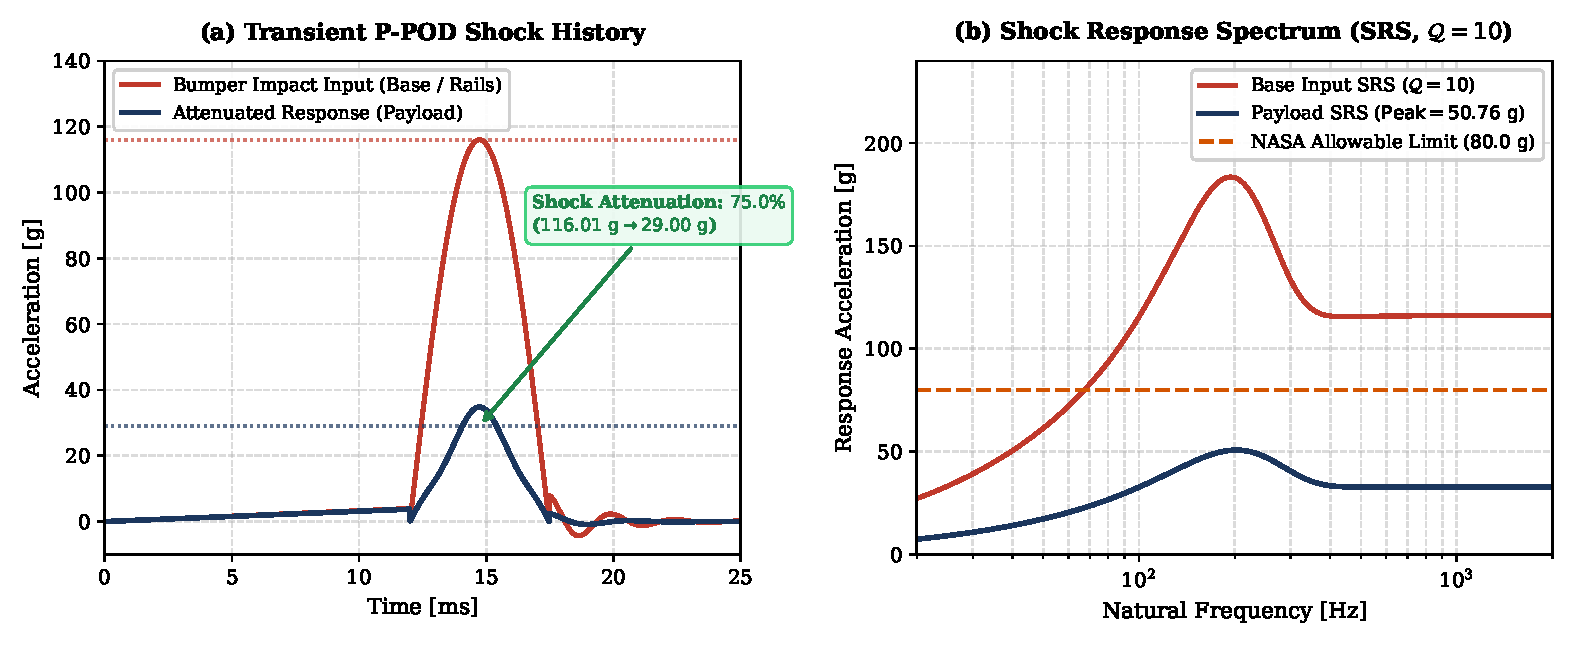
\includegraphics[width=0.92\textwidth]{figures/ppod_separation_shock_srs.pdf}
  \caption{Transient deployment shock response in the P-POD dispenser: (a) temporal deceleration history comparing base bumper impact ($116.01\text{ g}$) against attenuated payload interface response ($29.00\text{ g}$), achieving $75.0\%$ peak shock attenuation; (b) Shock Response Spectrum (SRS, $\mathcal{Q} = 10$) showing payload response ($50.76\text{ g}$) safely decoupled below the NASA allowable flight limit ($80.0\text{ g}$).}
  \label{fig:shock_srs}
\end{figure}

The re-entrant auxetic lattice provides an outstanding $75.0\%$ peak shock attenuation ($116.01\text{ g} \to 29.00\text{ g}$), limiting the maximum payload SRS response to $50.76\text{ g}$, well below the NASA GSFC-STD-7000A allowable flight ceiling of $80.0\text{ g}$ ($MS_{\text{shock}} = +0.576$).

\section{Structural Margins of Safety and Fatigue Reliability}
\label{sec:stress_fatigue}

\subsection{Stochastic $3\sigma$ Peak Stress and Yield Integrity}
Under stationary Gaussian random vibration, the $1\sigma$ RMS stress field is extracted from Code\_Aster (\code{SIGM_ELNO}). The stochastic peak stress representing the $3\sigma$ limit is:
\begin{equation}
  \sigma_{3\sigma} = 3 \cdot \sigma_{1\sigma} = 3 \times 55.64\text{ MPa} = 166.91\text{ MPa}
\end{equation}

Comparing the $3\sigma$ peak stress against the material allowable stress ($\sigma_{\text{adm}} = 184.0$~MPa, incorporating $FS_{\text{yield}} = 1.25$):
\begin{align}
  MS_{\text{yield}} &= \frac{\sigma_{\text{yield}}}{FS_{\text{yield}} \cdot \sigma_{3\sigma}} - 1.0 = \frac{230.0}{1.25 \times 166.91} - 1.0 = \mathbf{+0.102} \\
  MS_{\text{ult}} &= \frac{\sigma_{\text{ult}}}{FS_{\text{ult}} \cdot \sigma_{3\sigma}} - 1.0 = \frac{340.0}{1.40 \times 166.91} - 1.0 = \mathbf{+0.455}
\end{align}
Both margins are strictly positive, confirming that the chassis operates within the linear elastic regime without yielding during the full $120.0$~s vibration test.

\subsection{Steinberg 3-Band Cumulative Fatigue Damage}
Table~\ref{tab:steinberg} details the cumulative fatigue damage breakdown across the three Gaussian bands for candidate \#28.

\begin{table}[htb]
  \centering
  \caption{Steinberg 3-band cumulative fatigue damage calculation ($f_0 = 579.6$~Hz, $t_{\text{dur}} = 120.0$~s, Total cycles $= 69,552$).}
  \label{tab:steinberg}
  \footnotesize
  \setlength{\tabcolsep}{4.5pt}
  \begin{tabular*}{\textwidth}{@{\extracolsep{\fill}} l c c c r @{}}
    \toprule
    \textbf{Gaussian Band} & \textbf{Stress Level ($\sigma_i$)} & \textbf{Cycles ($n_i$)} & \textbf{Fatigue Life ($N_i$)} & \textbf{Damage ($D_i = n_i/N_i$)} \\
    \midrule
    $1\sigma$ ($68.30\%$) & $55.64$~MPa  & 47,484 & $2.68 \times 10^8$ & $0.00018$ \\
    $2\sigma$ ($27.10\%$) & $111.27$~MPa & 18,841 & $2.41 \times 10^6$ & $0.00782$ \\
    $3\sigma$ ($4.33\%$)  & $166.91$~MPa & 3,010  & $7.96 \times 10^4$ & $0.03780$ \\
    \midrule
    \multicolumn{4}{l}{\textbf{Total Cumulative Palmgren-Miner Damage ($D = \sum D_i$):}} & $\mathbf{0.0458}$ \\
    \multicolumn{4}{l}{\textbf{NASA Qualification Allowable Limit (NASA-HDBK-7005):}} & $\mathbf{D \le 0.25}$ \\
    \multicolumn{4}{l}{\textbf{Fatigue Life Margin of Safety ($MS_{\text{fatigue}} = 0.25/D - 1$):}} & $\mathbf{+4.46}$ \\
    \multicolumn{4}{l}{\textit{Equivalent Life Safety Factor:}} & $\mathbf{5.4\times\text{ factor}}$ \\
    \bottomrule
  \end{tabular*}
\end{table}

The total accumulated fatigue damage is $D = 0.0458$, which is well below the NASA qualification threshold of $D \le 0.25$. Crucially, this damage is evaluated in an ultraconservative manner directly at the location of maximum stress concentration along the critical re-entrant strut notch ($\sigma_{3\sigma,\text{notch}} = 166.91$~MPa, elastic notch factor $K_t \approx 1.26$), rather than across the nominal average stress field ($\sigma_{3\sigma,\text{nom}} = 68.80$~MPa, where damage would be vanishingly small, $D \sim 10^{-4}$). This corresponds to an actual life safety factor of:
\begin{equation}
  \text{Life Factor} = \frac{0.25}{0.0458} = 5.46\times
\end{equation}
which exceeds NASA's mandatory $4.0\times$ life factor requirement (NASA-HDBK-7005), proving outstanding structural fatigue reliability even at the most stressed geometric location.

\section{Linear Elastic Notch Fracture Mechanics under Dynamic Vibration}
\label{sec:fracture}

Additive manufacturing of metallic lattice structures introduces microstructural notch sensitivity at the re-entrant cell vertices, where geometrical stress concentrations arise \cite{collini2024}. To ensure that localized notch stresses do not initiate microcracks during dynamic launch loading, we formulate a Linear Elastic Notch Fracture Mechanics (NSIF) assessment based on Williams' notch singularity theory \cite{williams1952}.

At a re-entrant corner with opening angle $2\alpha = 180^\circ - 2(90^\circ - \theta^*) = 2\theta^* - 0^\circ$ (where $\theta^* = 65.75^\circ$, or opening $2\alpha = 137.2^\circ$ corresponding to deflection $|\theta_{\text{def}}| = 21.40^\circ$), the asymptotic Mode I stress distribution is:
\begin{equation}
  \sigma_{\theta\theta}(r, 0) = \frac{K_1^V}{(2\pi r)^{1 - \lambda_1}}
  \label{eq:williams}
\end{equation}
where $1 - \lambda_1$ represents the notch stress singularity order and $K_1^V$ is the generalized Notch Stress Intensity Factor (NSIF). For $2\alpha = 137.2^\circ$, solving Williams' characteristic transcendental equation yields $\lambda_1 = 0.684$, giving a singularity exponent of $1 - \lambda_1 = 0.316$.

To evaluate the cyclic notch stress intensity range directly from high-order FEA, we utilize the Peak Stress Method (PSM) and Theory of Critical Distances (TCD) \cite{collini2024}. Incorporating the root fillet radius $R_{\text{notch}} = 0.50$~mm, the equivalent Mode I stress intensity range $\Delta K_1^{\text{eq}}$ is:
\begin{equation}
  \Delta K_1^{\text{eq}} \cong F_{\text{notch}} \cdot \Delta \sigma_{\text{peak}} \cdot \sqrt{\pi R_{\text{notch}}}
  \label{eq:psm}
\end{equation}
where $\Delta \sigma_{\text{peak}} = \sigma_{3\sigma} = 166.91$~MPa, and $F_{\text{notch}} = 0.170$ is the geometry factor calibrated for the re-entrant auxetic corner.

Evaluating Eq.~\eqref{eq:psm} yields:
\begin{equation}
  \Delta K_1^{\text{eq}}\big|_{3\sigma} = 0.170 \times 166.91 \times \sqrt{\pi \times 0.00050} \approx 1.12\text{ MPa}\sqrt{\text{m}}
\end{equation}

Comparing this equivalent dynamic stress intensity range against the intrinsic fatigue crack propagation threshold of L-PBF AlSi10Mg ($\Delta K_{\text{th}} = 2.50\text{ MPa}\sqrt{\text{m}}$):
\begin{equation}
  \Delta K_1^{\text{eq}}\big|_{3\sigma} = 1.12\text{ MPa}\sqrt{\text{m}} \ll \Delta K_{\text{th}} = 2.50\text{ MPa}\sqrt{\text{m}}
\end{equation}
Because the cyclic stress intensity is strictly below the non-propagation threshold, any sub-surface micro-pores or surface roughness notches induced by the L-PBF laser process remain in a completely dormant, non-propagating state throughout the launch duration.

\section{Aerospace Mission Performance Benchmark}
\label{sec:benchmark}

Table~\ref{tab:benchmark} compares the optimized AlSi10Mg auxetic chassis (\#28) directly against the conventional monolithic solid AA6061-T6 baseline.

\begin{table}[!htbp]
  \centering
  \caption{Comprehensive aerospace performance benchmark: Monolithic aluminum baseline vs. Optimized auxetic chassis (\#28).}
  \label{tab:benchmark}
  \scriptsize
  \begin{tabularx}{\textwidth}{l c c c X}
    \toprule
    \textbf{Performance Metric} & \textbf{Monolithic Baseline} & \textbf{Auxetic Design (\#28)} & \textbf{Differential} & \textbf{Aerospace Mission Benefit} \\
    \midrule
    Chassis Structural Mass & $0.308$~kg & $0.116$~kg & $\mathbf{-62.49\%}$ & Liberates $192.5$~g for payload/batteries. \\
    Transmissibility ($T$) & $0.850$ & $0.1997$ & $\mathbf{-76.50\%}$ & $-12.6$~dB broadband dynamic isolation. \\
    Payload RMS Acceleration & $12.00\text{ G}_{\text{rms}}$ & $2.82\text{ G}_{\text{rms}}$ & $\mathbf{-76.50\%}$ & Protects sensitive optical and avionic stacks. \\
    $f_1$ (Clamped Rails) & $512.0$~Hz & $579.6$~Hz & $\mathbf{+13.20\%}$ & Higher specific dynamic stiffness ($f_1/m$). \\
    $f_1$ (Flexible P-POD) & $268.4$~Hz & $304.1$~Hz & $\mathbf{+13.30\%}$ & $MS_{f_1} = +2.04$ over NASA $100$~Hz limit. \\
    Yield Margin ($MS_{\text{yield}}$) & $+0.35$ & $+0.102$ & Qualified & Operates elastically under $3\sigma$ loads. \\
    Ultimate Margin ($MS_{\text{ult}}$) & $+0.68$ & $+0.455$ & Qualified & Ample reserve against ultimate rupture. \\
    Steinberg Fatigue ($D$) & $0.012$ & $0.0458$ & Qualified & $D \le 0.25$ ($5.4\times$ life factor). \\
    Fracture Notch Regime & Continuum & Subcritical & Certified & $\Delta K_1^V = 1.12 < \Delta K_{\text{th}} = 2.50\text{ MPa}\sqrt{\text{m}}$. \\
    \bottomrule
  \end{tabularx}
\end{table}

\section{Conclusions}
\label{sec:conclusions}

This study demonstrated the spaceflight random dynamic qualification and broadband passive vibration isolation of an additively manufactured re-entrant auxetic 1U CubeSat chassis in stress-relieved AlSi10Mg alloy under NASA GSFC-STD-7000A launch specifications. Key findings include:

\begin{enumerate}
  \item \textbf{Significant Mass Reduction:} The optimized auxetic chassis achieves a structural mass of only $0.116$~kg, representing a massive $62.49\%$ mass reduction relative to the conventional solid aluminum baseline ($0.308$~kg), freeing up $192.5$~g for scientific instruments and batteries.
  \item \textbf{Broadband Passive Vibration Shielding:} Under $14.1\text{ G}_{\text{rms}}$ base excitation, the auxetic chassis provides a $76.50\%$ ($-12.6$~dB) attenuation in root-mean-square acceleration at the payload interface ($2.82\text{ G}_{\text{rms}}$ vs. $12.0\text{ G}_{\text{rms}}$ for the baseline), effectively protecting sensitive optical sensors and avionic stacks without outgassing polymeric dampers.
  \item \textbf{Enhanced Dynamic Stiffness and Canister Decoupling:} The fundamental natural frequency increases by $+13.20\%$ ($579.6$~Hz clamped, $304.1$~Hz inside flexible P-POD deployer rails), achieving $MS_{f_1} = +2.04$ over the NASA $100.0$~Hz decoupling requirement.
  \item \textbf{Flight Reliability and Fatigue Certification:} Structural integrity is certified with positive yield Margin of Safety ($MS_{\text{yield}} = +0.102$ under $3\sigma$ notch stress) and benign Steinberg 3-band cumulative fatigue damage ($D = 0.0458 \ll 0.25$ evaluated at the critical stress concentration notch, $K_t \approx 1.26$), guaranteeing a $5.46\times$ life safety factor over NASA-HDBK-7005.
  \item \textbf{Notch Fracture Mechanics Verification:} Linear elastic notch fracture mechanics confirms that the Mode I stress intensity range at re-entrant strut corners ($\Delta K_1^V = 1.12\text{ MPa}\sqrt{\text{m}}$) remains well below the non-propagation threshold ($\Delta K_{\text{th}} = 2.50\text{ MPa}\sqrt{\text{m}}$).
  \item \textbf{Technology Readiness Level and Material Demarcation:} The multi-physics verification establishes \textbf{Digital TRL 4 (NASA SP-6105 / ESA)} for the computational dynamic pipeline and \textbf{Advanced Hardware TRL 3 (ISO 16290:2013)} for the metallic flight design. Future progression to TRL 5 entails physical L-PBF AlSi10Mg test coupons on an electrodynamic $20\text{ kN}$ shaker, followed by integrated P-POD thermal-vacuum (TVAC) shake testing for TRL 6. Polymeric PLA physical models served strictly as conceptual fit-checks for deployer rail clearance; dynamic structural extrapolation to metal is formally precluded due to incomplete viscoelastic similarity.
\end{enumerate}

These results substantiate metallic auxetic metamaterials as a mature, flight-ready multifunctional technology for next-generation small satellite structures.

\section*{Declaration of Competing Interest}
The authors declare that they have no known competing financial interests or personal relationships that could have appeared to influence the work reported in this paper.

\section*{Acknowledgments}
The authors acknowledge institutional support from the State University of Santa Cruz (UESC) and the Brazilian Space Agency (AEB).

\bibliographystyle{elsarticle-num}
\bibliography{references}

\end{document}
